\documentclass[11pt]{report}
\usepackage[a4paper,left=2cm,right=2cm,top=2cm,bottom=2cm,marginparwidth=2cm]{geometry}
\usepackage[T1]{fontenc}
%\usepackage{natbib}
\usepackage[style=apa, backend = biber]{biblatex}
\addbibresource{biblio.bib}
\usepackage{csquotes}
\usepackage[french]{babel}
\usepackage{
    setspace,
    %amsthm,
    graphicx,
    %svg,
    array,
    enumitem,
    tabularx,
    titlesec,
    tocloft
}
%\usepackage[hyphens]{url}   % permet de couper les URLs sur les tirets
%\usepackage{breakurl}  
\usepackage{wrapfig}
\usepackage[colorlinks=true,linkcolor=blue,citecolor=blue,urlcolor=blue]{hyperref}
\usepackage{amsmath} 



% Configuration des chemins
\graphicspath{{images/}}

% Configuration des tableaux
%\let\oldtabular\tabular
%\def\tabular{\footnotesize\oldtabular}

%\let\oldtabularx\tabularx
%\def\tabularx{\footnotesize\oldtabularx}

% Configuration des titres
\titleformat{\chapter}[hang]
    {\normalfont\Huge\bfseries}
    {\thechapter}
    {1em}
    {}

\titlespacing*{\chapter}
    {0pt}       % indentation à gauche
    {0.2em}    % espace au-dessus du titre
    {1.8em}       % espace après le titre
    
\titleformat{\paragraph}
    {\normalfont\normalsize\itshape}
    {\theparagraph}
    {1em}
    {}

\titlespacing*{\paragraph}
    {0pt}
    {3.25ex plus 1ex minus .2ex}
    {1.5ex plus .2ex}
    
\titlespacing*{\subsection}
    {0pt}
	{2.5ex plus 1ex minus .2ex}
	{1.5ex plus .2ex}

% Configuration de la table des matières
\setcounter{tocdepth}{3}


%%%%%%%%%%%%%%%%%%%%%%%%%%%%%%%%%%%%%%%%%%%%%%%%%%%%%%

\begin{document}

% Cacher numéro de page : à réafficher à l'intro
\pagenumbering{gobble}

\begin{titlepage}
    \centering
    % En-tête avec logos
    
\includegraphics[height=0.22\textwidth]{images/ens.pdf}
    \hspace{5pt}
    \raisebox{0.5\height}{\vrule width 1pt height 50pt}
    \hspace{5pt}
    
\includegraphics[height=0.22\textwidth]{images/R1.pdf}
    \vspace{1cm}

    % Informations institutionnelles
    \Large
    {\textbf{École normale supérieure de Rennes\\
    Département Sciences du sport et éducation physique}}
    \vspace{0.5cm}

    {\textbf{Diplôme de l'ENS -- 1\textsuperscript{ère} année\\
    Année universitaire 2025-2026\\
    Discipline : STAPS}}
    \vspace{1cm}

    {\textit{Mémoire en Sciences de la Vie et de la Santé}}
    \vspace{1cm}

    % Titre du mémoire
    \rule{\linewidth}{0.5mm} \\[0.5cm]
    \huge \textbf{Identification des marqueurs de motricité fine les plus caractéristiques des TSA chez l'enfant : Approche bayésienne par projection prédictive 
} \\[0.5cm]
    \rule{\linewidth}{0.5mm} \\[1cm]

    % Auteurs et encadrant
    \Large
    \textbf{Présenté par :}\\
    Romain MARTINIE
    \vspace{1cm}

    \textbf{Encadrants :}\\
    Laetitia FRADET (Université de Bretagne-Sud) \\ \& \\ Germain FAITY (ENS, département 2SEP)
\end{titlepage}

\onehalfspacing
\newpage
\null
\newpage

% Remerciements
%\chapter*{Remerciements}
%\newpage

% Attestation sur l'honneur
\chapter*{Attestation sur l'honneur}
Je soussigné, Romain MARTINIE, atteste sur l'honneur de ne pas avoir eu recours au plagiat et que ce mémoire de recherche est le résultat d'un travail personnel. La rédaction de ce travail a été effectuée avec l'aide d'intelligence artificielle générative (modèle Claude Sonnet 4.6 : assistance dans le code, les formulations et correction de la langue).
\newpage


% Sommaire
\tableofcontents
\newpage

% Liste des abrévations
%\chapter*{Liste des abrévations}
%\newpage

% Tables des illustrations
%\chapter*{Tables des illustrations}
\begingroup
\let\clearpage\relax
\listoffigures
\listoftables
\endgroup

%\chapter*{Table des annexes}
%\begin{itemize}[label={},leftmargin=1.5em]
%\end{itemize}
%\newpage




% Introduction
\chapter{Introduction}

\pagenumbering{gobble}
\pagestyle{plain}
\pagenumbering{arabic}
\setcounter{page}{1}
En France, en 2003, les registres régionaux estimaient la prévalence des troubles du spectre de l'autisme (TSA) chez les enfants de moins de sept ans à 4,1 pour 1 000 \parencite[p.10]{HAS2018_TSA}. Cette valeur est probablement sous-évaluée, car les formes plus modérées échappent souvent aux dispositifs d'identification \parencite[p.10]{HAS2018_TSA}. Par ailleurs, le nombre de diagnostics tend à augmenter \parencite{zeidan_global_2022} et la reconnaissance institutionnelle des TSA s'accroît\footnote{Comme en témoigne en France la \textit{Stratégie nationale pour les troubles du neurodéveloppement 2023-2027}, \url{https://handicap.gouv.fr/nouvelle-strategie-nationale-pour-les-troubles-du-neurodeveloppement-autisme-dys-tdah-tdi}}. Les retards dans le diagnostic peuvent dépasser un an entre la première prise de contact et la restitution du diagnostic en France dans le cadre d'un Centre de Ressources Autisme (CRA) \footnote{IGAS. (2015). \textit{Évaluation des Centres de ressources autisme (CRA) en appui de leur évolution} (p. 37). \url{https://igas.gouv.fr/sites/igas/files/files-spip/pdf/2015-124R-2.pdf}}, illustrant la difficulté à diagnostiquer les individus autistes.

\bigskip

Le diagnostic, posé par un psychiatre, repose principalement sur les altérations de la communication et des interactions sociales, ainsi que sur les comportements stéréotypés et les intérêts restreints \parencite[p.~56–58]{apa_diagnostic_2022}. Cette approche présente des limites en pratique clinique, pouvant conduire à des biais (par exemple liés au genre, voir Section \ref{sec:norme}) ou expliquer en partie les retards dans la prise en charge par les CRA.

\bigskip

Pour autant, la littérature montre que les TSA s'accompagnent de caractéristiques motrices qui ne sont pas exploitées pour le diagnostic. Ces particularités apparaissent pourtant précocement, parfois dès les premiers mois de vie, voire avant les signes sociaux atypiques \parencite{Zwaigenbaum2015Oct, AlSagheer2018Sep}. Parallèlement, des corrélats neuronaux pourraient expliquer ces manifestations motrices et le phénotype autistique dans son ensemble (voir Section \ref{sec:bases_neuro}). Ces observations suggèrent que les caractéristiques motrices pourraient ainsi constituer des marqueurs précoces du développement autistique.


\bigskip

Ce mémoire s'inscrit dans la continuité des travaux réalisés dans le cadre du projet "\textit{Identifier et caractériser les déficits moteurs associés aux troubles du spectre autistique}", dont une partie des données a déjà été exploitée dans la thèse de \textcite{benchekri_mieux_2024}. En mobilisant une approche bayésienne, ce mémoire vise à identifier les variables de motricité fine les plus caractéristiques des enfants autistes, afin de proposer des pistes d'amélioration dans la compréhension et le diagnostic des TSA.



%En France, en 2003, les registres régionaux estimaient la prévalence des troubles du spectre de l'autisme (TSA) chez les enfants de moins de sept ans à 4,1 pour 1 000 \parencite[p.10]{HAS2018_TSA}. Cette valeur est considérée comme sous-évaluée puisque les formes plus modérées échappent souvent aux dispositifs d'identification \parencite[p.10]{HAS2018_TSA}. Malgré une tendance à l'augmentation du nombre de diagnostics \parencite{zeidan_global_2022} et une reconnaissance institutionnelle croissante \footnote{Comme en témoigne en France la \textit{Stratégie nationale pour les troubles du neurodéveloppement 2023-2027}, \url{https://handicap.gouv.fr/nouvelle-strategie-nationale-pour-les-troubles-du-neurodeveloppement-autisme-dys-tdah-tdi}}, la compréhension des TSA reste partielle. Le diagnostic est posé par des psychiatre et se base principalement sur altérations de communication/interactions sociales et comprotements térétotypés et intérêts marqués \parencite[p.~56–58]{apa_diagnostic_2022}. Les retards dans le diagnostic peuvent dépasser 1 an d'attente entre 1ere prise de contact (déjà pas évidente à obtenir) et restitution du diagnostic pour CRA. \footnote{\url{https://comprendrelautisme.com/les-acteurs/les-centres-de-ressources-autisme/}}, ce qui illustre les difficultés à identifier précocement ces troubles.

\bigskip

%Or, la littérature montre que les TSA s'accompagnent aussi de corrélats neuronaux (voir Section \ref{sec:bases_neuro}) qui pourraient expliquer le phénotype autistique, et des spécifictés motrices (voir Section \ref{sec:controle_moteur}). Ces composantes motrices, souvent négligées, apparaissent pourtant précocement, parfois dès les premiers mois de vie, voire avant les signes sociaux atypiques \parencite{Zwaigenbaum2015Oct, AlSagheer2018Sep}. Leur méconnaissance limite la capacité à identifier et comprendre précocement les TSA.

\bigskip

%Ce mémoire se propose d'examiner ces composantes motrices comme des marqueurs précoces du développement autistique. En mobilisant une approche bayésienne, il vise à sélectionner les variables de motricité fine les plus caractéristiques des enfants autistes, au sein de plusieurs tâches de motrcité fine. Afin de contribuer à une meilleure compréhension et à l'amélioration du diagnostic des TSA.


\bigskip

%Ce mémoire s'inscrit dans la continuité des travaux réalisés dans le cadre du projet "\textit{Identifier et caractériser les déficits moteurs associés aux troubles du spectre autistique}", dont une partie des données a déjà été exploitée dans la thèse de \textcite{benchekri_mieux_2024}. En mobilisant une approche bayésienne, ce mémoire vise à identifier les variables de motricité fine les plus caractéristiques des enfants autistes, afin de proposer des pistes d'amélioration dans la compréhension et le diagnostic des TSA.


\chapter{Revue de littérature}
% Corps du texte
\section{Les troubles du spectre de l'autisme (TSA)}
\subsection{Définition}
Les troubles du spectre de l'autisme (TSA) sont des troubles neurodéveloppementaux caractérisés par des difficultés persistantes dans la communication et les interactions sociales, ainsi que par des comportements et intérêts restreints ou répétitifs \parencite[p.~56–58]{apa_diagnostic_2022}.
Ce trouble apparait pendant la période du développement, en général à la petite enfance. L'appellation "spectre" reflète une forte hétérogénéité individuelle au-delà des critères centraux de la communication et des comportements répétitifs \parencite{oms_classification_2018}. Ainsi, les TSA peuvent également se manifester à travers une déficience intellectuelle, des troubles du langage ou des troubles moteurs \parencite[p.~62]{apa_diagnostic_2022}, et sont souvent accompagnés de comorbidités \parencites[p.~67–68]{apa_diagnostic_2022}{lord_autism_2018}.

%\subsection{Etiologie}
%Rajouter rapidement Etiologie ??

%Principalement génétique, héréditaire à 80\,\%
%+ facteurs environnementaux

\subsection{Prévalence et comorbidités} \label{sec:prev_comor}
La prévalence des TSA est estimée à environ 1\,\% dans le monde, bien que les chiffres varient selon les études et aient tendance à augmenter avec le temps en raison d'une hausse des demandes de diagnostic \parencite{zeidan_global_2022, brugha_epidemiology_2011, Elsabbagh2012Apr}.
Les garçons sont généralement plus nombreux que les filles, avec un ratio masculin/féminin variant autour de 4 \parencite{zeidan_global_2022}, malgré des biais genrés compliquant l'évaluation (voir Section~\ref{sec:norme}). Les TSA seraient associés à une probabilité accrue de déficience intellectuelle (DI), mais la proportion n'est pas connue \parencite{zeidan_global_2022}.
%est importante puisque les chiffres vont de 0\,\% à 70\,\% \parencite{zeidan_global_2022} + 2e source.

Par ailleurs, les TSA s'accompagnent fréquemment de comorbidités psychiatriques. Chez l'enfant, environ 45\,\% présentent par exemple au cours de leur vie un trouble déficitaire de l'attention avec hyperactivité (TDAH), 42\,\% un trouble anxieux et 14\,\% une dépression \parencite{Micai2023Dec}. Chez l'adulte, ces proportions sont respectivement de l'ordre de 22\,\%, 28 à 42\,\% et 34\,\% \parencite{hollocks_anxiety_2019, Micai2023Dec} et sont donc supérieures à celles de la population générale. On y retrouve en effet autour de 4\,\% pour le TDAH \parencite{Popit2024Oct, Song2021Feb}, 9\,\% pour le trouble anxieux \parencite{Kessler2012Aug} et 29\,\% pour la dépression \parencite{Kessler2012Aug, Hu2022May}.

\medskip

La prévalence et la diversité des comorbidités psychiatriques observées invitent donc à un diagnostic le plus précoce possible. En ce sens, quand est-ce que les premières caractéristiques autistiques émergent-elles ? Demeurent-elles stables tout au long du développement ?

\subsection{Apparition du phénotype et trajectoires développementales}
Dès les premiers mois de vie, des signes précoces du phénotype autistique apparaissent. Alors, dès l'âge d'un an, peuvent être observées des difficultés dans les premières interactions sociales, ainsi que des comportements répétitifs ou stéréotypés \parencite{Webb2009Apr,Tanner2021Mar,Zwaigenbaum2015Oct}. Un contrôle moteur atypique, que ce soit au niveau de la motricité globale ou de la  motricité fine, est également décrit dès 6 à 12 mois \parencite{Estes2015Jul,Zwaigenbaum2015Oct}. 

Pour autant, les trajectoires développementales sont hétérogènes. En effet, si le diagnostic de l'autisme est stable dans le temps, on observe une grande hétérogénéité entre les études \parencite{Bieleninik2017Sep}. De plus, bien que l'expression du phénotype autistique tende, en moyenne, à diminuer de l'enfance à l'adolescence \parencite{Waizbard-Bartov2022Nov}, entre 20\,\% et 49\,\% des enfants avec un TSA présentent néanmoins une régression dans les domaines du langage ou de la communication sociale \parencite{Webb2009Apr}. Cette évolution dépend alors de variables comme l'environnement ou la présence ou non de déficience intellectuelle \parencite{Waizbard-Bartov2022Nov}.

\medskip

Ainsi, l'apparition précoce du phénotype autistique et son évolution avec l'âge invitent à s'intéresser à la population pédiatrique. Par ailleurs, la présence d'un éventail de caractéristiques aussi diversifiées dès les premiers stades soulève la question de leurs bases neurobiologiques. Quelles altérations cérébrales pourraient expliquer la diversité des manifestations observées chez les enfants avec TSA ?

\section{Bases neuronales des TSA} \label{sec:bases_neuro}

Les bases neuronales des TSA peuvent être comprises non pas comme l'altération d'une région cérébrale unique, mais comme un ensemble d'anomalies fonctionnelles et morphologiques affectant le cerveau à une échelle globale. Sans prétendre à l'exhaustivité, nous présenterons ici un aperçu des connaissances actuelles afin de situer les altérations cérébrales susceptibles de sous-tendre les caractéristiques observées chez les enfants avec TSA.

\subsection{Bases structurelles} \label{sec:bases_struct}

Sur le plan structurel, les analyses de morphométrie voxel‐à‐voxel (VBM) mettent en évidence un ensemble d'altérations de la matière grise chez les personnes présentant un TSA. Il a notamment été rapporté des réductions de volume dans le cortex cingulaire antérieur et médio-préfrontal, dans l'insula ainsi que dans le cervelet postérieur \parencite{Guo2024Apr}. Ces anomalies sont souvent convergentes entre mesures fonctionnelles et morphologiques \parencite{Patriquin2016Oct}. De plus, il a été mis en évidence des volumes plus faibles du putamen, de l'amygdale, du noyau accumbens et du pallidum. Ces différences sous-corticales semblent relativement stables au cours du développement, tandis que les altérations corticales tendent à s'atténuer à l'âge adulte \parencite{vanRooij2017Nov}.

\subsection{Altérations fonctionnelles}

En imagerie fonctionnelle, les études au repos montrent, chez les sujets autistes, notamment une tendance à une hypoactivation dans l'insula gauche, du cortex cingulaire antérieur et médial préfrontal (ACC/mPFC), ainsi que dans l'aire temporale inférieure droite, accompagnée d'une hyperactivation du précuneus et de l'aire motrice supplémentaire \parencite{Guo2024Apr}. Des altérations concernent également le \textit{default mode network} (DMN), où la connectivité entre le cortex préfrontal et le cortex cingulaire postérieur/precuneus apparaît réduite chez les individus avec TSA, ce qui pourrait expliquer certains troubles dans la cognition sociale \parencite{Sato2019Aug}. Des anomalies comparables touchent aussi les régions du "cerveau social" hors DMN, notamment l'amygdale \parencite{Sato2019Aug}, dont la connectivité affaiblie avec le cortex préfrontal ventromédian est corrélée à la sévérité des symptômes socio-affectifs \parencite{Kleinhans2015Dec}. On observe également une dépendance du profil d'activation en fonction du type de tâche mobilisée : les tâches non sociales montrent un recrutement anormal de l'ACC dorsal et de l'aire motrice supplémentaire, tandis que les tâches sociales révèlent par exemple une hypoactivation du cortex cingulaire postérieur 
\parencite{DiMartino2008Nov}.

Le chevauchement des différences neuronales avec des régions impliquées dans le contrôle moteur, telles que le cervelet, les ganglions de la base et le cortex préfrontal, pourrait expliquer les difficultés motrices fréquemment observées chez les sujets avec TSA. En effet, des lésions du cervelet pourraient perturber le contrôle en  \textit{feedforward} ou la coordination sensori-motrice \parencite{Manto2012Jun}. De même, les ganglions de la base pourraient être liés à l'apparition de mouvements stéréotypés \parencite{Groenewegen2003}. %lié à tourettes's

\medskip
Ainsi, les données de neuroimagerie révèlent des caractéristiques neuronales distribuées plutôt que localisées, affectant des régions impliquées dans la cognition sociale, la régulation émotionnelle et le contrôle moteur. Le chevauchement de ces anomalies avec celles observées dans d'autres troubles du neurodéveloppement ou pathologies complexifie leur interprétation \parencite{Guo2024Apr, Lukito2020Mar}.
Parmi les régions altérées, on retrouve de façon récurrente des structures en lien avec la motricité, notamment le cervelet ou les ganglions de la base. Cette implication dans un trouble défini par des critères socio-cognitifs interroge la place des troubles moteurs dans le phénotype autistique. Alors, comment les connaissances issues des modèles cérébraux actuels s'intègrent-elles, ou non, dans les outils de diagnostic existants, et quelles en sont les limites ?

\section{Diagnostic des TSA : outils, validité, et limites méthodologiques}
Malgré la mise en évidence progressive de différences neuronales suggérant l'existence de marqueurs non seulement sociaux mais aussi moteurs chez les personnes présentant un TSA, la recherche et la pratique clinique se sont historiquement centrées sur les dimensions psycho-socio-cognitives du trouble \parencite{cook_movement_2016}. Pour autant, le diagnostic des TSA reste complexe en raison d'un chevauchement symptomatique (voir section~\ref{sec:prev_comor}) et neuronal (voir section~\ref{sec:bases_struct}) avec d'autres troubles du neurodéveloppement ou d'autres pathologies. 

Actuellement, le diagnostic repose sur une évaluation clinique intégrant l'observation comportementale, l'histoire développementale et les informations parentales, selon un consensus pluridisciplinaire considéré comme le \textit{gold standard} \parencites[p.~52]{HAS2018_TSA}{Randall2018Jul, Hirota2023Jan, falkmer_diagnostic_2013, Woolfenden2012Jan}. Un nombre important d'outils standardisés pour assister le diagnostic ont été proposés \parencites[p.~51]{HAS2018_TSA}{falkmer_diagnostic_2013, Randall2018Jul}. Ainsi, aujourd'hui, les outils standardisés considérés comme la référence et les plus utilisés sont l'\textit{Autism Diagnostic Interview, Revised} (ADI-R) et l'\textit{Autism Diagnostic Observation Schedule, 2e édition} (ADOS-2) \parencite{Hirota2023Jan, frigaux_ladi-r_2019}.



\subsection{Outils comportementaux de référence} %(ADOS/ADI-R)}

L'ADOS-2 est un outil standardisé et semi-structuré d'observation directe, basé sur l'évaluation de la communication, l'interaction sociale, le jeu et les comportements répétitifs chez les personnes suspectées de TSA \parencite{Lord2012ADOS2}. Il se compose de 4 modules adaptés à l'âge et au niveau de langage de l'individu \parencite{Lord2012ADOS2}. L'ADI-R, quant à lui, prend la forme d'un entretien semi-structuré mené auprès des parents ou aidants d'enfants et d'adultes, portant sur la trajectoire développementale de l'individu \parencite{Lord1994Oct}. 

\medskip

Il convient alors de s'interroger sur la validité de ces outils diagnostiques : le statut de référence qui leur est attribué est-il justifié par leur validité ?

\subsection{Validité et questionnement du statut de référence}

Chez les enfants, l'ADI-R possède une sensibilité de l'ordre de 60 à 70\,\% et une spécificité d'environ 80\,\% \parencite{Lebersfeld2021Nov, Fulceri2025Jun, dosSantos2024Screening, Randall2018Jul}. Cependant, ces résultats cachent une incertitude très élevée, avec des plages de sensibilité s'étendant de 19 à 100\,\% et une spécificité comprise entre 50\,\% et 100\,\% \parencite{Lebersfeld2021Nov, Fulceri2025Jun}. L'ADOS-2 montre dans la même population une sensibilité légèrement plus importante, de l'ordre de 90\,\%, et une spécificité autour de 70-80\,\% avec incertitude notable mais plus faible que pour l'ADI-R (sensibilité : 77–100\,\% ; spécificité : 44–100\,\%) \parencite{Lebersfeld2021Nov, Fulceri2025Jun}. %L'usage combiné des deux outils pourrait améliorer la validité au prix d'une baisse de sensibilité. C'est en effet ce qui est observé pour la combinaison de l'ADI-R et de l'ADOS (1ère édition) \parencite{Randall2018Jul, Lebersfeld2021Nov}.

En termes de fiabilité inter‑juges, des accords élevés sont rapportés pour l'ADI-R, avec des taux compris entre 80 et 90\,\% \parencite{Lord1994Oct, Zander2017}. Il en va de même pour l'ADOS-2, bien que la fiabilité dépende fortement de l'expérience de l'évaluateur, avec des taux d'accord variant de 50 à 86\,\% selon les modules et l'expérience de l'évaluateur \parencite{Kamp-Becker2018Sep}.

Un biais circulaire doit également être pris en compte : les études de validation de ces outils s'appuient généralement sur un diagnostic de référence posé par une équipe pluridisciplinaire, laquelle intègre déjà les résultats de l'ADOS/ADOS-2 et de l'ADI-R dans son évaluation.

Enfin, les performances varient aussi selon les profils cliniques : la spécificité de l'ADI-R peut, par exemple, tomber à 57\,\% chez les adultes sans déficience intellectuelle \parencite{adamou_predicting_2021}. Ainsi, bien qu'efficaces, les outils standardisés sont sujets à une validité incertaine et hétérogène en fonction des populations. Cette hétérogénéité questionne la dépendance de ces outils à des normes développementales, mais aussi sociales, qu'il convient d'interroger.

\subsection{Ancrage normatif des outils de diagnostic}\label{sec:norme}

Les outils de diagnostic possèdent un biais de genre marqué : les filles sont régulièrement sous-diagnostiquées \parencite{Gupta2025Jan, Lai2023Dec, Rea2023Jul}. Ce phénomène s'explique en partie par des facteurs socioculturels et par la construction genrée des outils et des critères diagnostiques. En effet, la plupart des tests ont été élaborés à partir de cohortes majoritairement masculines, et certains comportements typiques des TSA peuvent être socialement tolérés, voire valorisés, chez les filles \parencite{Lai2023Dec}. De plus, la difficulté d'application des outils standardisés auprès de populations présentant des particularités sensorielles, telles qu'une déficience visuelle ou auditive \parencite{Hirota2023Jan}, ou encore la nécessité de traduire ces outils et d'en valider ces traductions constituent des limites supplémentaires.

\medskip

En outre, les outils actuellement utilisés pour le diagnostic des TSA présentent des biais %méthodologiques et sociaux 
qui conduisent à une sous-identification récurrente de certaines populations, notamment féminines, et une validité incertaine. Dans cette perspective, une approche fondée sur le contrôle moteur, en complément des outils actuellement utilisés, pourrait contribuer à réduire certains de ces biais. En effet, la motricité et notamment la motricité fine est moins susceptible d'être influencée par les différences de genre, de handicap, ou de contexte culturel que les interactions sociales. De plus, les altérations motrices observées chez les personnes autistes sont corrélées avec les caractéristiques centrales des TSA comme les difficultés sociales ou de communication \parencite{hocking_what_2017}. 

\section{TSA et contrôle moteur : caractérisation de la motricité fine}
\label{sec:controle_moteur}
Dès les premières étapes du développement, les enfants présentant un TSA montrent majoritairement des déficiences dans les évaluations standardisées du développement moteur, qu'il s'agisse de la motricité globale ou de la motricité fine \parencite{hocking_what_2017}. %Des particularités motrices ont notamment été rapportées dans des tâches mobilisant la motricité fine, telles que l'écriture ou le pointage et la saisie manuelle \parencite{hocking_what_2017}.
Toutefois, tous les enfants avec TSA ne présentent pas nécessairement de déficiences motrices \parencite{hocking_what_2017}. Ainsi, plutôt que de ne prendre en compte uniquement ces difficultés motrices, il apparaît pertinent d'examiner les particularités de la motricité globale comme fine chez les enfants avec TSA. Dans cette optique, nous faisons ici le choix de nous intéresser à la motricité fine, à travers l'étude des modèles de pointage, de saisie manuelle et d'écriture.
%il apparaît plus judicieux dans une perspective diagnostique et de compréhension d'évoquer les caractéristiques générales et atypiques de la motricité fines des TSA. Nous aborderons alors modèles de pointage/écriture ?

\subsection{Pointage et saisie manuelle}\label{sec:pointage}
%def pointage ?

La littérature met en évidence, chez les enfants présentant un TSA, une tendance à une augmentation du temps de mouvement lors des tâches de pointage et de saisie manuelle \parencite{benchekri_mieux_2024, Glazebrook2006Jul, forti_motor_2011}, bien que ce résultat ne soit pas systématiquement observé \parencite{Papadopoulos2012Jan, Rinehart2006Aug}, ainsi qu'une diminution de la fluidité du mouvement \parencite{benchekri_mieux_2024}. Alors, cette diminution de la vitesse pourrait être interprétée soit comme la cause d'une réduction de la fluidité du mouvement, soit, au contraire, comme sa conséquence, à l'image de ce qui a été observé chez des adultes atteints du syndrome parkinsonien \parencite{benchekri_mieux_2024}.
De plus, il a été rapporté une augmentation du temps d'élaboration de la commande motrice \parencite{Glazebrook2006Jul, Rinehart2006Aug}, pouvant refléter un dysfonctionnement des ganglions de la base similaire à celui observé chez les patients parkinsoniens \parencite{Rinehart2006Aug}.

Il est important de noter que ces différences sont modulées par des variables de confusion, notamment le quotient intellectuel (QI) ou la complexité de la tâche \parencite{Mari2003Feb}. Ainsi, les enfants présentant un TSA associé à un QI plus faible que la moyenne tendent à exécuter les mouvements plus lentement que ceux ayant un QI plus élevé \parencite{Mari2003Feb}.


\subsection{Écriture} \label{sec:ecriture}
%def écriture, stroke ?
Chez les enfants présentant un TSA, on peut retrouver des difficultés marquées dans l'écriture. On retrouve notamment une diminution de la lisibilité globale et une détérioration de la formation des lettres \parencite{Kushki2011Dec, Handle2022Oct}. Au niveau moteur, l'écriture se caractérise par une vitesse d'exécution ralentie et une fluidité de mouvement plus faible \parencite{benchekri_mieux_2024, kangarani-farahani_motor_2024, Handle2022Oct}.
Il peut être considéré que ces caractéristiques résulteraient notamment d'une altération de la coordination visuomotrice, les enfants présentant un TSA s'appuieraient en effet préférentiellement sur le \textit{feedback} proprioceptif \parencite{benchekri_mieux_2024, kangarani-farahani_motor_2024, shafer_visual_2021}. %L'augmentation du contrôle en \textit{feedback} entraînant plus de corrections et une donc une diminution de la fluidité.
\medskip


Nous avons pu voir que des caractéristiques spécifiques de la motricité fine chez les enfants autistes sont mises en évidence au sein de tâches de pointage ou d'écriture, et ne se limitent pas aux déficits fonctionnels observés par les tests standardisés. Une approche consistant d'abord en une classification, puis en la détermination des profils moteurs, pourrait permettre une caractérisation plus fine de ces différences. Cette démarche contribuerait à la compréhension du phénotype moteur des TSA ainsi que des mécanismes neurofonctionnels sous-jacents. En effet, ces caractéristiques motrices, cohérentes avec les altérations des structures impliquées dans le contrôle moteur (voir section \ref{sec:bases_neuro}), apparaissent comme des manifestations potentiellement informatives du fonctionnement cérébral des TSA. Une description précise de ces profils moteurs pourrait ainsi favoriser l'identification de marqueurs pertinents, utiles tant pour améliorer le diagnostic précoce des TSA que pour approfondir la compréhension de ce trouble, en offrant la possibilité de repérer des profils neurofonctionnels équivalents.
Dans cette perspective, la littérature récente mobilise des approches fondées sur l'apprentissage automatique pour, d'une part, caractériser la motricité fine des individus avec un TSA, et, d'autre part, classifier les profils neurotypiques de ceux des enfants présentant un TSA.

\subsection{Apport des approches par apprentissage automatique}

\subsubsection{Classification en fonction de variables motrices}\label{sec:classification}

Tout d'abord, la littérature montre de manière convergente la faisabilité d'une classification des TSA par des approches d'apprentissage automatique appliquées à des tâches de motricité fine. Les précisions sont généralement comprises entre 70 et 90\,\% selon la tâche et le modèle utilisés, qu'il s'agisse de tâches d'imitation gestuelle au niveau de la main \parencite{Li2017Aug, FulinLiu2024Apr, vabalas_applying_2020}, de saisie manuelle \parencite{crippa_use_2015,Simeoli2021May,Milano2023May,Su2024Dec, freud_effective_2025, cavallo_identifying_2021}, de dessin \parencite{Emanuele2021Aug}, ou de pointage \parencite{Anzulewicz2016Aug, Luongo2024Apr, Doctor2025Jul}.

\subsubsection{Caractérisation de la motricité fine}
Par ailleurs, les modèles issus de ces études mettent en évidence des différences dans les vitesses, accélérations et dans la variabilité des trajectoires et amplitudes, traduisant des mouvements moins fluides chez les enfants avec TSA \parencite{Simeoli2021May, Milano2023May, Li2017Aug, Doctor2025Jul}. Il a été proposé que les enfants avec TSA auraient une moindre dépendance au \textit{feedback} sensoriel, en particulier visuel, et des stratégies de contrôle davantage en boucle ouverte \parencite{Emanuele2021Aug, crippa_use_2015, Anzulewicz2016Aug}, ce qui est cohérent avec les conclusions des études plus observationnelles (voir Sections \ref{sec:pointage}, \ref{sec:ecriture}).

%lles décrivent la motricité des TSA mais de part le fait que les tâches et variables aient été choisie a priori on sait pas si elles sont représentatives, on sait pas si elles sont les plus caractéristiques + on peut pas les comparer entre elles !!

\medskip

Pour autant, les approches par apprentissage statistique demeurent à un stade de preuve de concept \parencite{Doctor2025Jul}. Bien qu'il soit possible d'extraire de l'information pertinente pour la classification à partir de tâches de motricité fine, les variables de confusion, telles que l'âge ou la présence ou non de déficience intellectuelle, peuvent biaiser l'apprentissage des modèles et ne sont pas toujours prises en compte \parencite{cavallo_identifying_2021}. De plus, les échantillons étudiés sont souvent relativement faibles comparés au nombre de \textit{features}, ce qui entraîne un risque de sur-apprentissage%[source,]
. Enfin et surtout, la validation d'une approche automatique reste limitée par une forte hétérogénéité méthodologique, tant au niveau des tâches que des \textit{features} extraites, ce qui empêche la constitution d'un modèle entraîné sur un grand volume de données et donc pleinement généralisable.

Face à cette hétérogénéité, l'identification des variables motrices les plus caractéristiques permettrait d'orienter la collecte de données pour le développement d'outils diagnostics basés sur la motricité. De plus, dans une perspective de modélisation \textit{utile}, cela permettrait de formuler des hypothèses sur les systèmes neuronaux sous-jacents impliqués chez les sujets TSA. Par exemple, si les variables les plus discriminantes reflètent principalement des processus de planification, cela suggérerait une implication prédominante des ganglions de la base et permettrait de mobiliser les connaissances issues de la maladie de Parkinson pour mieux comprendre les mécanismes autistiques \parencite{Rinehart2006Aug}.

% Problématique, objectifs et hypothèses
\chapter{Problématique, objectifs et hypothèses}

\section{Problématique}
La revue de la littérature met en évidence le besoin de mieux comprendre les TSA et de pouvoir les diagnostiquer précocement. Bien que l'on possède des connaissances sur les bases neuronales, la compréhension des TSA et les outils de diagnostic actuels restent largement imparfaits. En ce sens, une caractérisation de la motricité fine des TSA, notamment par des approches computationnelles, pourrait être une stratégie pertinente pour combler ces limites. Toutefois, ces approches ne sont pas cliniquement exploitées. Une limite majeure que l'on peut noter est l'hétérogénéité des variables mesurées et des tâches utilisées. Ainsi, déterminer les marqueurs moteurs les plus caractéristiques des TSA constituerait une avancée pour la compréhension et le diagnostic de ce trouble. 

\bigskip

Nous nous proposons d'identifier, parmi un ensemble de tâches de motricité fine, les marqueurs moteurs les
plus caractéristiques chez l'enfant avec TSA, dans l'objectif de mieux comprendre les altérations motrices associées et de contribuer, à titre exploratoire, au développement d'outils diagnostiques complémentaires à ceux utilisés aujourd'hui.

\section{Objectifs}
%L'objectif principal de ce mémoire est de déterminer les marqueurs moteurs les plus caractéristiques des TSA chez l'enfant, à partir de données issues de tâches de motricité fine. 
À l'aide d'analyses adaptées à un contexte de forte dimensionnalité, ce travail vise, d'une part, à améliorer la compréhension des TSA en reliant les marqueurs moteurs identifiés aux corrélats neuronaux décrits dans la littérature. D'autre part, il cherche à identifier une tâche ou un ensemble de variables de motricité fine présentant un fort pouvoir discriminant, afin d'évaluer l'existence de différents profils moteurs au sein de la population TSA. Cette approche pourrait constituer une base pour de futures études à plus large échelle, visant le développement d'outils de classification automatique en complément du diagnostic actuel.


\section{Hypothèses}
Sur la base de la littérature et des questionnements précédents, nous faisons l'hypothèse qu'il sera possible de classifier les enfants présentant un TSA par rapport aux enfants neurotypiques avec une précision de l'ordre de 70 à 90\,\% -- avec une sensibilité et spécificité équilibrée -- à partir de l'ensemble des variables motrices issues des différentes tâches, et ce, sans sur-apprentissage. Nous supposons par ailleurs qu'un sous-ensemble restreint, correspondant aux variables les plus discriminantes, sera suffisant pour classifier les deux groupes avec des performances comparables à celles obtenues avec l'ensemble complet des marqueurs% (typiquement <1 sd ELPD/qq \%)
. Enfin, nous faisons l'hypothèse que les variables motrices les plus discriminantes présenteront des liens cohérents avec les corrélats neurophysiologiques décrits dans la littérature, principalement le cervelet et les ganglions de la base, et qu'elles seront donc majoritairement associées à la fluidité et à l'accélération du mouvement.


%hypothèses trop générales ?
%partie moteur/neuro trop rapide ?


\chapter{Matériel et méthodes}

Les données analysées dans ce mémoire sont issues des travaux de la thèse de \textcite{benchekri_mieux_2024}, dont nous rappelons 
ici les éléments de protocole nécessaires à la compréhension 
de la démarche statistique. 


\section{Protocole expérimental}

\subsection{Population}
L'étude a inclus des enfants âgés de 6 à 12 ans, répartis en deux groupes : des enfants avec un trouble du spectre de l'autisme (TSA) et des enfants à développement "typique" (TD). Pour les enfants TSA, le diagnostic a été validé cliniquement par les équipes médicales des structures partenaires où ils étaient suivis, et objectivé par un score seuil à l'ADI-R et/ou à l'ADOS.

\subsection{Dispositif et tâches motrices}

Le protocole comprenait des tâches organisées de la façon suivante : motricité fine, motricité globale, puis oculométrie. Parmi l'ensemble des tâches proposées, quatre étaient en lien avec la motricité fine et ont donc donné lieu aux variables analysées dans ce mémoire. Les données motrices ont été recueillies à l'aide d'une tablette graphique et d'un stylet \footnote{Tablettes Yiynova MSP19U ou Huion 19GT-190 en fonction du site de recueil des données (19 pouces échantillonnage 200 Hz, 1024 points de pression, temps de retour 5ms)}, sur quatre sites : Bordeaux, La Rochelle, Limoges, Poitiers.


\subsubsection{Anticipation pointage}

La tâche d'anticipation pointage (PA) consistait à pointer successivement deux cibles avec le stylet, en partant d'un carré de 0,5~cm de côté. La première cible, d'un diamètre de 2~cm, était présentée horizontalement à 10~cm de la zone de départ, à gauche ou à droite. La seconde cible était placée au-dessus de la première, à 14~cm de celle-ci, et pouvait présenter deux diamètres : 2~cm ou 0,5~cm, correspondant respectivement aux conditions facile et difficile (voir figure~\ref{fig:PA}).


\begin{figure}[ht]
	\centering
	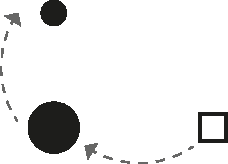
\includegraphics[scale=1.4]{PA.pdf}
	\caption[Configuration expérimentale pour la réalisation de la tâche d'Anticipation Pointage]{Configuration expérimentale pour la réalisation de la tâche d'Anticipation Pointage. La première cible pouvait apparaître à droite ou à gauche. La seconde cible est ici représentée en condition difficile (cible petite). N'est pas à l'échelle.}
	\label{fig:PA}
\end{figure}

\subsubsection{Anticipation écriture}

La tâche d'anticipation écriture (ll\_ln) consistait à recopier avec le stylet et par-dessus un modèle, deux digrammes (\textit{ll} et \textit{ln}) présentés en écriture cursive, sans espace entre les deux lettres (voir figure~\ref{fig:ll_ln}). On parle d'anticipation car le sujet devait planifier son geste d’écriture en fonction de la lettre suivante (\textit{l} ou \textit{n}) avant d’avoir terminé la première. 

\begin{figure}[ht]
	\centering
	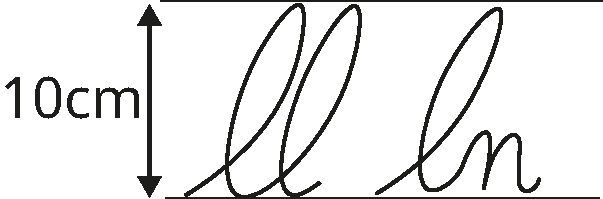
\includegraphics[scale=0.8]{ll_ln.pdf}
	\caption{Représentation des visuels utilisés pour la réalisation de la tâche d'Anticipation Écriture}
	\label{fig:ll_ln}
\end{figure}

\subsubsection{Isochronie}

Pour la tâche d'isochronie (Epow), le participant devait recopier, avec le stylet et par-dessus un modèle, la lettre \textit{e} selon cinq tailles différentes. Pour chaque taille, cinq essais consécutifs étaient réalisés avant de passer à la taille suivante (voir figure~\ref{fig:epow}).


\begin{figure}[ht]
	\centering
	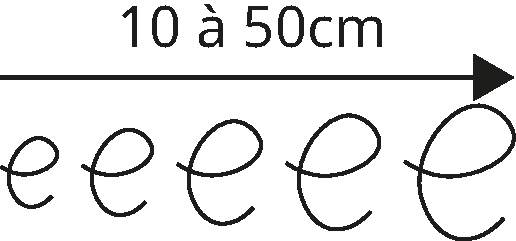
\includegraphics[scale=0.8]{epow.pdf}
	\caption[Représentation des visuels utilisés pour la réalisation de la tâche d'isochronie]{Représentation des visuels utilisés pour la réalisation de la tâche d'isochronie. Pour chaque taille, 5 essais étaient réalisés. N'est pas à l'échelle.}
	\label{fig:epow}
\end{figure}

\subsubsection{Pointage simple}

La tâche de Pointage Simple (PS) correspondait à une tâche de Fitts \parencite{Fitts1954}. Le participant devait pointer une cible avec le stylet dès son apparition, le plus rapidement possible et sans lever le stylet, en partant d'un carré de 0,5~cm de côté. Quatre niveaux de difficulté ont été définis par l'indice de difficulté ID, calculé selon la formule suivante :

\[
\text{ID} = \log_2\!\left(\frac{2A}{w}\right)
\]

où $A$ désigne la distance entre le centre de chaque cible et $w$ la largeur de la cible. Les paramètres associés à chaque niveau de difficulté sont présentés dans le tableau~\ref{table:IDfitts}.


\begin{table}[ht]
	\centering
	\begin{tabularx}{0.65\textwidth}{X X X}
		\hline \textbf{ID} & \textbf{Distance $A$ (cm)} & \textbf{Taille $w$ (cm)} \\ \hline
		3 & 8 & 2 \\
		4 & 16 & 2 \\
		5 & 8 & 0,5 \\
		6 & 16 & 0,5 \\ \hline
	\end{tabularx}
	\caption{Paramètres utilisés lors de la tâche de Fitts}
	\label{table:IDfitts}
\end{table}


\section{Description du jeu de données}

%Les données ont été collectées sur quatre sites cliniques à l'aide d'un système de capture de mouvement Vicon%(+ ref mais pas la ref). 
Au total, 66 enfants TSA et 62 enfants TD ont été rencontrés. Après traitement des données, le jeu de données final retenu pour les analyses comprend 45 enfants TSA et 49 enfants TD.
%\medskip 
À partir des enregistrements issus des quatre tâches, 142 variables motrices ont été extraites, auxquelles s'ajoutent l'âge et le sexe de chaque enfant, soit 144 variables prédictives (\textit{features}) au total. On peut répartir ces variables en trois catégories : des variables cinématiques et temporelles brutes (distances, vitesses, durées\dots), des variables dérivées (SPARC, curve index\dots) et des variables spécifiques aux tâches (indice d'isochronie, pente de la loi de Fitts\dots). Une description complète de l'ensemble des variables est disponible en \hyperref[table:annexe_description_var]{Annexe A}.

\medskip

Le ratio variables/observations ($D/n = 144/94 \approx 1.5$) est supérieur à~1. L'analyse statistique est donc dans un cas de grande dimension%Bellman fléeau ?
. Ce constat motive le recours à un cadre régularisant pour déterminer les variables les plus caractéristiques.



\section{Cadre de l'inférence bayésienne}
L'inférence bayésienne repose sur le théorème de Bayes, qui exprime la distribution \textit{a posteriori} des paramètres $\theta$ du modèle conditionnellement aux données observées $y$ :
\[
p(\theta \mid y) \propto p(y \mid \theta)\, p(\theta)
\]


où $p(y \mid \theta)$ désigne la vraisemblance des données et $p(\theta)$ la distribution \textit{a priori} sur les paramètres. Contrairement à l'approche fréquentiste (cadre "classique"), les paramètres ne sont pas estimés ponctuellement mais caractérisés par une distribution de probabilité, qui quantifie explicitement l'incertitude sur leurs valeurs. L'inférence porte ainsi sur $p(\theta \mid y)$ et non sur la probabilité des données sous l'hypothèse nulle. Il est important de noter que les probabilités sont ici considérées de façon \textit{épistémique} : elles modélisent l'incertitude des paramètres et non leur fréquence.

Les approches fondées sur les tests d'hypothèse nulle et le seuil de significativité $p < 0.05$ font l'objet de critiques méthodologiques majeures \parencite{Amrhein2019Mar, Ioannidis2005Aug}. Elles encouragent notamment le raisonnement binaire, entrainent une inflation des erreurs de type I et ne permettent pas de quantifier l'incertitude sur les paramètres d'intérêt. Dans le contexte de ce mémoire où $p > n$, on s'attend à une grande incertitude sur les paramètres et à un risque important d'erreurs de type I dans un cadre fréquentiste. 

\medskip 

Ainsi, une méthodologie bayésienne lève ces limitations en fournissant une distribution de probabilité complète par paramètre, en s'affranchissant du problème des comparaisons multiples \parencite{Gelman2009Jul} %(à lire)
 et en intégrant la régularisation via les distributions \textit{a priori} (voir section~\ref{sec:prior}). 

\medskip 

En pratique, la distribution \textit{a posteriori} n'est pas calculable analytiquement dans le cas général. Elle est approchée par simulation via des méthodes de Monte Carlo par chaînes de Markov (MCMC), qui permettent d'approximer la distribution de $p(\theta \mid y)$ en obtenant des échantillons de celle-ci. Une limite importante de la méthodologie appliquée est donc le coût computationnel qui est supérieur aux approches fréquentistes classiques, bien que les implémentations actuelles rendent ce coût élevé mais acceptable pour les dimensions considérées ici.


 
 \section{Cadre interprétatif de la sélection}
 La sélection de variables est réalisée selon un critère prédictif (voir section~\ref{sec:critere}) : une variable est considérée comme informative si sa présence dans le modèle améliore la capacité à prédire l'appartenance au groupe TSA ou TD sur de nouvelles observations \parencite{projpred}. Nous considérerons que si une variable est prédictive, alors elle reflète une caractéristique motrice différenciant les deux groupes sans que cela constitue une preuve de causalité. Ainsi, si un sous-ensemble de variables prédit aussi bien que le modèle complet, les variables exclues sont soit du bruit, soit redondantes, c'est-à-dire qu'elles partagent une information mutuelle 
 élevée \footnote{
 	Au sens de la théorie de l'information, l'information mutuelle entre deux variables aléatoires 
 	$X$ et $Y$ est définie par :
 	\[
 	I(X\,;Y) = H(X) + H(Y) - H(X,Y)
 	\]
 	où $H$ désigne l'entropie de Shannon. Elle mesure la quantité d'information partagée entre $X$ et $Y$, et vaut zéro si et seulement si $X$ et $Y$ sont indépendantes.
 } avec les variables déjà sélectionnées sans pour autant être du bruit. La redondance n'est pas limitée aux relations linéaires d'ordre~1 (corrélation) : des dépendances non linéaires entre variables peuvent également conduire à l'exclusion d'une variable par ailleurs pertinente.

\medskip 

 Ces considérations impliquent que la liste des variables sélectionnées constitue un point de départ pour l'exploration clinique et expérimentale et non un ensemble exhaustif ou définitif de marqueurs du TSA. 

\section{Prétraitement des données}

Trois sujets présentant des valeurs manquantes ont été exclus de l'analyse. Un sujet supplémentaire a été exclu sur la base d'un critère de valeur aberrante : toute observation présentant un score $|z| > 5$ sur au moins une variable était candidate à l'exclusion. L'exclusion a été confirmée après vérification en unités naturelles et examen du contexte de la tâche. Au total, 90 sujets ont donc été retenus pour l'analyse (46 TD et 44 TSA).

\medskip

L'ensemble des variables a ensuite été centré et réduit (moyenne et écart-type estimés sur l'échantillon), de façon à les ramener à une échelle commune. Cette normalisation repose sur des estimateurs fréquentistes, ce qui constitue une légère entorse à la cohérence bayésienne stricte mais était néanmoins nécessaire pour l'application de distributions a priori régularisantes comparables entre coefficients (voir section~\ref{sec:prior}).

\section{Modèle de référence}
\subsection{Régression logistique bayésienne}

Le modèle de référence est une régression logistique bayésienne. La variable à prédire $y_i \in \{0, 1\}$ indique l'appartenance de l'individu $i$ au groupe TSA ($y_i = 1$) ou TD ($y_i = 0$). Le modèle est défini tel que : 

\begin{align*}
	y_i &\sim \text{Bernoulli}(\pi_i), \quad i = 1, \dots, n \\
	\text{logit}(\pi_i) &= \alpha + \sum_{j=1}^{D} \beta_j x_{ij}, 
	\quad j = 1, \dots, D
	\label{eq:vraisemblance}
\end{align*}

où $\pi_i = P(y_i = 1 \mid x_i)$ est la probabilité d'appartenir au groupe TSA, $\alpha$ l'ordonnée à l'origine, $\beta_j$ le coefficient associé à la variable $x_{ij}$, et $D$ le nombre total de variables. La fonction logit, définie par $\text{logit}(\pi) = \log(\pi / (1-\pi))$, assure que $\pi_i \in ]0,1[$. Géométriquement, le modèle définit un hyperplan qui sépare les groupes TD et TSA dans l'espace des \textit{features} dont la distance signée détermine la probabilité d'appartenance à chaque groupe.

\subsection{Spécification des priors}\label{sec:prior}

Dans le cadre bayésien, les distributions a priori peuvent jouer un rôle analogue à la régularisation en statistique fréquentiste en contraignant les coefficients vers zéro, d'autant plus quand il y a peu de données. Un \textit{a priori} (prior) gaussien centré correspond à une pénalité ridge ($L_2$) tandis qu'un prior laplacien correspond à une pénalité lasso ($L_1$). Ces deux approches présentent cependant des limitations dans le régime $p > n$ : le prior gaussien écrase uniformément tous les coefficients sans produire de sparsité (coefficient à 0), tandis que le prior laplacien tend à trop contraindre les effets importants.

\medskip 

Le prior \textit{Regularized Horseshoe} (RHS) \parencite{Piironen2017Jul} est proposé pour dépasser ces limites dans un cadre bayésien, pour les problèmes de sélection de variables en grande dimension. Il repose sur une décomposition en deux niveaux de régularisation :
\begin{align*}
	\beta_j &\sim \mathcal{N}(0,\, \tau^2 \tilde{\lambda}_j^2) \\
	\tilde{\lambda}_j^2 &= \frac{c^2 \lambda_j^2}{c^2 + \tau^2 \lambda_j^2} \\
	\lambda_j &\sim \mathrm{C}^+(0, 1), \qquad 
	\tau \sim \mathrm{C}^+(0, \tau_0) \\
	c^2 &\sim \mathrm{Inv\text{-}Gamma}\!\left(\frac{\nu}{2},\, 
	\frac{\nu s^2}{2}\right)
\end{align*}

où $\mathrm{C}^+$ désigne la distribution demi-Cauchy. Le paramètre $\tau$ joue le rôle de \textit{shrinkage global} : il pousse l'ensemble des coefficients vers zéro. Le paramètre $\lambda_j$ joue le rôle de \textit{shrinkage local} : il permet aux coefficients présentant un signal suffisant d'échapper à cet écrasement. Le terme $c^2$, issu d'une distribution \textit{Inverse-Gamma} de paramètres $(\nu/2, \nu s^2/2)$ avec $\nu = 4$ et $s = 2$ (valeurs recommandées par \cite{Piironen2017Jul}), régularise les coefficients importants en bornant leur variance \textit{a priori}.

L'hyperparamètre $\tau_0$, qui calibre le shrinkage global en fonction de la sparsité attendue, est défini par :

\[
\tau_0 = \frac{p_0}{D - p_0}\,\frac{\sigma}{\sqrt{n}}
\]

où $p_0$ est le nombre de variables a priori supposées prédictives, $D$ le nombre total de variables, $n$ la taille d'échantillon, et $\sigma$ un facteur d'échelle dans le cadre de la régression logistique. Conformément aux recommandations de \textcite{Piironen2017Jul} pour la régression logistique, $\sigma$ est fixé à 2. Nous posons $p_0 = 10$, reflétant l'hypothèse que seul un petit nombre de variables parmi les $D = 144$ est suffisant pour discriminer les deux groupes. Ce choix est exploratoire et sa sensibilité est évaluée dans la section~\ref{sec:sensi}.

L'intercept $\alpha$ reçoit un prior Student-t faiblement informatif, centré en zéro :

\[
\alpha \sim \mathrm{Student\text{-}t}(\nu=7,\, \mu=0,\, \sigma=2.5)
\]



\subsection{Critères de validité du modèle}\label{sec:validite}

La performance prédictive du modèle est évaluée par validation croisée \textit{leave-one-out}\footnote{La validation croisée LOO correspond à, à chaque itération d'apprentissage/validation, réaliser l'apprentissage sur $n - 1$ observations et la validation sur l'unique observation restante.}\break (LOO-CV), approchée par l'estimateur PSIS-LOO (\textit{Pareto Smoothed Importance Sampling Leave-One-Out}) \parencite{Vehtari2015Jul}. Il estime l'\textit{expected log pointwise predictive density} (elpd), définie telle que :
% pas besoin d'aller dans les détail de l'estimateur PSIS imo, trop technique pour rien
\[
\text{elpd}_{\text{loo}} = \sum_{i=1}^{n} 
\log p(y_i \mid y_{-i})
\]

où $p(y_i \mid y_{-i})$ désigne la probabilité assignée par le modèle ajusté sur les $n-1$ observations restantes à la vraie classe de l'observation $i$. L'elpd est donc la somme des log-probabilités prédites pour chaque observation mise de côté tour à tour : plus elle est élevée, meilleure est la capacité du modèle à généraliser à de nouvelles données. L'elpd constitue le critère principal de comparaison entre modèles.

\medskip 

La fiabilité de l'approximation PSIS-LOO est contrôlée par les diagnostics $\hat{k}$ de Pareto : pour chaque observation $i$, un $\hat{k} > 0.7$ signale que l'approximation est peu fiable pour cette observation et que l'estimation de l'elpd doit être interprétée avec précaution \parencite{Vehtari2015Jul}. La précision de classification (\textit{accuracy}) %, \texttt{pctcorr} dans \texttt{projpred}) %SACHANT QUE J'AI PAS ENCORE PARLÉ DE PROJPRED A VOIR)
est rapportée comme critère complémentaire pour faciliter l'interprétation clinique des résultats. Elle est définie comme la proportion d'observations correctement classées, la classe prédite étant celle de probabilité maximale selon le modèle \parencite{projpred}.


\subsection{Diagnostics MCMC}
Il est nécessaire de vérifier la convergence des chaînes de Markov avant toute inférence, sans quoi les résultats risquent de ne pas être valides. Quatre chaînes de chacune 4000 itérations ont été simulées, dont 2000 de préchauffage (\textit{warmup}), soit 8000 échantillons post-warmup au total. %Le paramètre \texttt{adapt\_delta} a été fixé à 0.95 (valeur par défaut : 0.8) afin de prévenir l'apparition de transitions divergentes (indicateur de difficultés d'exploration de la distribution \textit{a posteriori}). 
La convergence est évaluée par le critère $\hat{R}$ de Gelman-Rubin. Une valeur $\hat{R}$ < 1.01 et une taille d'échantillon effective > 400 pour l'ensemble des paramètres sont retenues comme seuil de convergence \parencite{Vehtari2019Mar}. Ces diagnostics sont complétés par un examen visuel des traceplots, des graphiques d'autocorrélation et des distributions marginales \textit{a posteriori} (histogrammes et densités). %Compte tenu du nombre de paramètres, la checklist WAMBS complète n'est pas appliquée intégralement \parencite{Depaoli2017Jun} (exemple de diagnostics disponible en Annexe XXX).
 
\subsection{Vérifications prédictives (\textit{Predictive Checks)}}

Enfin, la validité du modèle a été évaluée par des vérifications prédictives (\textit{Predictive Checks}). Un \textit{Prior Predictive Check} a d'abord permis de s'assurer que les distributions \textit{a priori} ne contraignaient pas le modèle vers des prédictions extrêmes avant l'observation des données. Après ajustement, un \textit{Posterior Predictive Check} a été réalisé en comparant la distribution des données observées aux données simulées par le modèle. Le \textit{Posterior Predictive Check} montre que le modèle reproduit la proportion des classes (TSA/TD) sans pour autant présenter une certitude extrême et évite ainsi le surapprentissage. Les graphiques sont présentés en \hyperref[fig:ppc]{Annexe B}.


\section{Sélection par projection prédictive}
\subsection{Principe de cv varsel}
La sélection par projection prédictive \parencite{Piironen2018Oct} est une méthode de sélection de variables en fonction d'un modèle de référence, ici le modèle logistique bayésien complet ajusté sur l'ensemble des variables. Ce modèle constitue un plafond de performance prédictive : l'objectif est d'identifier le sous-modèle le plus parcimonieux dont la performance prédictive n'est pas inférieure à celle du modèle de référence (voir section~\ref{sec:critere} pour le critère de sélection).

\medskip

Le modèle de référence est d'abord ajusté sur l'ensemble des données et sa distribution \textit{a posteriori} est obtenue par MCMC. Une recherche forward est ensuite conduite : les variables sont ajoutées une à une au sous-modèle, en sélectionnant à chaque étape la variable qui minimise la divergence de Kullback-Leibler\footnote{
	La divergence de Kullback-Leibler, notée $D_{\text{KL}}$, est souvent décrite comme une mesure de la distance entre deux distributions de probabilité. Formellement, avec $P$ et $Q$ des densités de probabilité :
	\[
	D_{\text{KL}}(P \| Q) = \int p(x)\,\log\frac{p(x)}{q(x)}\,\mathrm{d}x	\]
}  entre les prédictions du sous-modèle projeté et celles du modèle de référence. La projection consiste à trouver, pour chaque taille de sous-modèle, les paramètres qui reproduisent au mieux le comportement prédictif du modèle de référence. Une fois le sous-modèle sélectionné, une inférence finale est conduite sur ce sous-modèle restreint.

\medskip 

La performance prédictive de chaque sous-modèle est évaluée par \texttt{cv\_varsel} avec \texttt{validate\_search = TRUE} \parencite{projpred}. Une LOO-CV est réalisée dans laquelle, à chaque fold, la recherche forward est réappliquée sur les $n-1$ observations d'entraînement. La performance à chaque étape (chaque \textit{fold} de LOO-CV pour chaque taille de sous-modèle $k$ testée) est définie par l'elpd approximé par PSIS-LOO. La performance finale du sous-modèle sélectionné est évaluée sur l'observation exclue. % Cela permet de corriger le biais de sélection lié à la recherche forward.
La fréquence à laquelle une variable est incluse dans le sous-modèle de taille $k$ à travers les folds permet de constituer une mesure de stabilité de la sélection.

\subsection{Critère de sélection}\label{sec:critere}

Le critère principal de sélection est l'elpd estimé par PSIS-LOO (voir section~\ref{sec:validite}). Pour chaque taille de sous-modèle $k$, l'écart à la performance du modèle de référence est quantifié par la différence $\Delta \text{elpd}_k=\text{elpd}_k - \text{elpd}_{ref}$ négative ou nulle par construction. La taille du sous-modèle retenu est déterminée principalement par la règle des $1\,\widehat{SE}$ (erreur standard)  \parencite{Piironen2018Oct} : le sous-modèle le plus parcimonieux tel que $|\Delta\text{elpd}_k| \leq \widehat{SE}(\Delta\text{elpd}_k)$, c'est-à-dire dont l'écart au modèle de référence reste inférieur à son erreur standard estimée. Ce critère est confirmé visuellement par le critère du coude sur la courbe $\Delta \text{elpd}_k$ et par la stabilité de sélection des variables. La précision est également rapportée mais la sélection de modèle est décidée par l'application des critères sur l'elpd.


\section{Screening par comparaison de modèles et sélection sur la tâche PA}
L'application de la sélection par projection prédictive sur le modèle global (144 variables) se heurte à une incertitude élevée sur l'estimation de l'elpd liée au ratio $D/n$ important. En l'absence de coude net dans la courbe $\Delta\text{elpd}_k$, il n'est pas possible d'identifier un sous-ensemble de variables de manière fiable à partir du modèle complet (voir section~\ref{sec:sel_global}).

\medskip

Pour contourner cette limite, le modèle global est décomposé en quatre sous-modèles de référence, un par tâche motrice (PA, ll\_ln, Epow, PS). Chaque sous-modèle est ajusté indépendamment avec le même prior RHS et la même procédure MCMC que le modèle global, à l'exception de $p_0 = 5$, ce qui reflète le moindre nombre de variables ($\tau_0$ recalculé en fonction, voir section~\ref{sec:prior}). La performance prédictive de chaque sous-modèle est estimée par PSIS-LOO et les $\hat{k}$ de Pareto sont rapportés pour chaque modèle. La comparaison des elpd entre sous-modèles et avec le modèle global est conduite par \texttt{loo\_compare} \parencite{loo}.

\medskip 

La tâche PA présente un elpd dont l'écart au modèle global reste inférieur à $1\,\widehat{SE}$ (voir section~\ref{sec:sel_PA}), ce qui satisfait le critère de sélection défini en section~\ref{sec:critere}. Elle est donc retenue comme tâche candidate pour la sélection par projection prédictive, son sous-modèle constituant le nouveau modèle de référence ($D_\text{PA} = 24$). 


\section{Analyse de sensibilité}\label{sec:sensi}
La sensibilité des résultats au choix de $p_0$ a été évaluée en réajustant le modèle de référence complet ($D=144$) avec trois valeurs : $p_0 \in \{5, 10, 20\}$, et le modèle de référence PA ($D=24$) avec $p_0 \in \{3, 5, 10\}$. Pour chaque valeur, $\tau_0$ est recalculé en conséquence (voir section~\ref{sec:prior}) et la procédure \texttt{cv\_varsel} est réappliquée. La stabilité des variables sélectionnées, de la taille du sous-modèle retenu et des coefficients des variables est examinée pour chacun des scénarios.
% + idem refaire une sensibilité avec p0 = 2 5 ou 10 sur PA ?


\section{Environnement logiciel}
Les analyses ont été conduites sous R version 4.5.3 \parencite{R}. Le modèle bayésien a été ajusté par l'algorithme de Monte Carlo hamiltonien implémenté dans \texttt{rstanarm} (version 2.32.1) \parencite{rstanarm}. La sélection par projection prédictive a été conduite avec le package \texttt{projpred} (version 2.10.0.9000) \parencite{projpred}. La validation croisée LOO et les diagnostics $\hat{k}$ de Pareto ont été calculés avec le package \texttt{loo} (version 2.9.0.9000) \parencite{loo}. La reproductibilité des résultats est assurée par une graine aléatoire (\texttt{123}). La robustesse du modèle de référence a été confirmée en vérifiant la stabilité des résultats avec une graine alternative (\texttt{1234}). L'ensemble des données et du code nécessaire à l'application de la méthodologie et de la compilation du mémoire est disponible au lien suivant : \texttt{\url{https://github.com/rmartinie/memoire-tsa-motricite-fine-bayesien}}.



\chapter{Résultats}

\section{Sélection sur le modèle global : limites de l'approche} \label{sec:sel_global}

\subsection{Courbe elpd et sélection des variables}

La procédure \texttt{cv\_varsel} a été appliquée sur le jeu de données complet, avec un nombre maximum de variables fixé à $k = 15$. Ce plafond a été validé en répétant la procédure avec $k = 25$, qui ne produit pas d'amélioration supplémentaire ni de l'elpd ni de l'\textit{accuracy}.  % à reformuler, ici ou en méthode ?

\medskip 

La courbe elpd (figure~\ref{fig:elpd_ref}) présente une première difficulté d'interprétation. En effet, selon le critère strict de l'erreur standard, le modèle à une seule variable est statistiquement équivalent au modèle complet, en raison d'une incertitude élevée sur les différences d'elpd. L'examen visuel de la courbe et les taux de sélection par \textit{fold} suggèrent néanmoins de retenir quatre variables, sélectionnées avec une stabilité respective de 0.99, 0.91, 0.97 et 0.93 (voir \hyperref[fig:stab_ref]{Annexe C} pour le détail par variable).

\begin{figure}[ht]
	\centering
	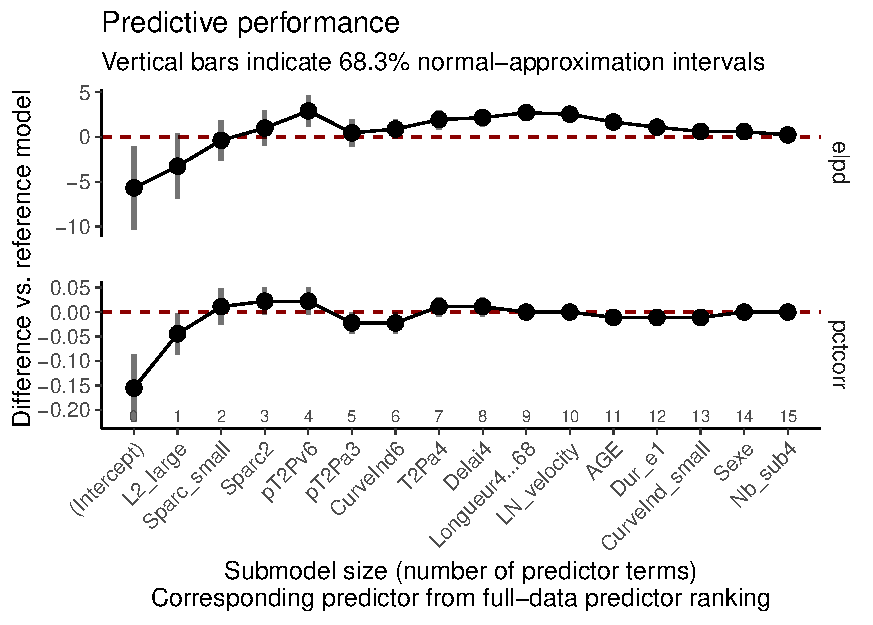
\includegraphics[scale=1]{elpd_ref.pdf}
	\caption[Courbes elpd et \textit{accuracy} issues du modèle de référence global]{Courbes de l'elpd et de l'\textit{accuracy} issues du modèle de référence global, en fonction du nombre de variables incluses dans le sous-modèle, obtenues par projection prédictive avec validation croisée. Chaque point représente la différence d'elpd/d'\textit{accuracy} entre le sous-modèle et le modèle de référence. Les barres d'erreur indiquent l'incertitude à $\pm 1$ erreur standard. Une différence proche de zéro indique des performances prédictives équivalentes au modèle de référence global.}
	\label{fig:elpd_ref}
\end{figure}


Le sous-modèle à quatre variables retenu est \texttt{L2\_large}, \texttt{Sparc\_small}, \texttt{Sparc2} et \texttt{pT2Pv6}. \texttt{L2\_large} correspond à la  distance parcourue de la première à la seconde cible lors de la tâche PA en condition "facile" (cible large). \texttt{Sparc\_small} et \texttt{Sparc2} sont des mesures de SPARC\footnote{Le SPARC (\textit{SPectral ARC length}) est défini comme la longueur de l'arc spectral de la vitesse du mouvement :	$\text{SPARC} = -\int_{0}^{\omega_c} \sqrt{\left(\frac{1}{\omega_c^2} + \frac{\mathrm{d}\hat{V}(\omega)} 		{\mathrm{d}\omega}\right)^2}\,\mathrm{d}\omega$, où $\hat{V}(\omega)$ est la transformée de Fourier de la vitesse et $\omega_c$ la fréquence de  coupure. Le SPARC est négatif. Une valeur plus proche de zéro indique un mouvement plus fluide \parencite{Balasubramanian2015Dec}.} (\textit{Spectral Arc Length}, mesure de fluidité) mesurée lors de la tâche PA et Epow, respectivement. Enfin, \texttt{pT2Pv6} correspond au temps pour atteindre le pic de vitesse (\textit{time to peak}) mesuré lors de la tâche PS avec $\text{ID} = 6$. 

\medskip 

Les estimations \textit{a posteriori} sont présentées dans la table~\ref{table:inf_full} pour les valeurs quantitatives et la figure~\ref{fig:mcmc_areas_ref} pour les distributions qualitatives des courbes de densité. Si la taille d'effet reste toujours très incertaine, la probabilité de direction est très forte pour chacune des 4 variables sélectionnées ce qui indique une faible incertitude quant au signe des effets. 

\medskip 

Les performances prédictives du sous-modèle sont comparables à celles du modèle de référence (sous-modèle vs référence ; elpd : $-54.61$ vs $-57.52$, \textit{accuracy} : 0.678 vs 0.656).  La matrice de confusion montre une classification modérée, avec 13 faux négatifs (classifié TD au lieu de TSA) et 12 faux positifs (classifié TSA au lieu de TD) sur 90 observations. L'\textit{accuracy} globale restant inférieure au seuil de 0.70, la capacité prédictive du modèle de référence est elle-même limitée, ce qui invite à la prudence dans l'interprétation des variables sélectionnées. Par ailleurs, le modèle ne montre pas de signe de surapprentissage.

\begin{figure}[ht]
	\centering
	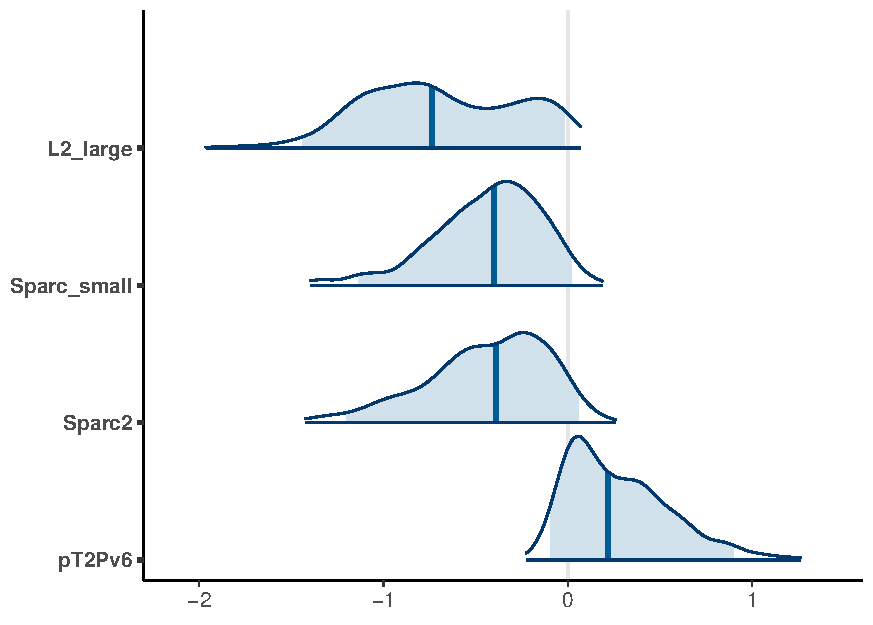
\includegraphics[scale=0.9]{mcmc_areas_cvvs_ref.pdf}
	\caption[Distributions \textit{a posteriori} du sous-modèle réduit à partir du modèle de référence global]{Distributions \textit{a posteriori} des coefficients de régression du sous-modèle à quatre variables à partir du modèle de référence global. Pour chaque paramètre, la barre verticale bleue indique la médiane \textit{a posteriori} et la zone bleue représente l'intervalle de crédibilité à 95\,\% (IC$_{95\%}$). Conditionnellement au modèle et	aux données, la valeur du paramètre a 95\,\% de chance de se situer dans cet intervalle.}
	\label{fig:mcmc_areas_ref}
\end{figure}

\begin{table}[ht]
	\centering
	\begin{tabular}{lcccc}
		\hline
		& Médiane & $\text{IC}_{95\%}$ & $\text{P}(\beta_j < 0)$ & $\text{P}(\beta_j > 0)$ \\
		\hline
		Intercept      &  0.035 & $[-0.468 \,;\, 0.541]$ & 0.443 & 0.558 \\
		L2\_large      & -0.738 & $[-1.442 \,;\, -0.018]$ & 0.978 & 0.023 \\
		Sparc\_small   & -0.400 & $[-1.137 \,;\, 0.020]$ & 0.970 & 0.030 \\
		Sparc2         & -0.392 & $[-1.201 \,;\, 0.059]$ & 0.955 & 0.045 \\
		pT2Pv6         &  0.216 & $[-0.095 \,;\, 0.898]$ & 0.130 & 0.870 \\
		\hline
	\end{tabular}
	\caption[Estimations \textit{a posteriori} du sous-modèle réduit à partir du modèle de référence global]{Estimations \textit{a posteriori} des coefficients du sous-modèle à quatre variables à partir du modèle de référence global. La médiane et l'intervalle de crédibilité à 95\,\% (IC$_{95\%}$) résument la distribution \textit{a posteriori} de chaque coefficient~; $\text{P}(\beta_j < 0)$ et $\text{P}(\beta_j > 0)$ indiquent la probabilité \textit{a posteriori} que le coefficient soit négatif ou positif, respectivement (probabilité de direction).}
	\label{table:inf_full}
\end{table}


%\begin{tabular}{lrr}
%	\hline
%	& 0 & 1\\
%	\hline
%	0 & 34 & 13\\
%	1 & 12 & 31\\
%	\hline
%\end{tabular}

\subsection{Diagnostics MCMC et approximation PSIS-LOO}
Les diagnostics MCMC à travers les \textit{traceplots}, les fonctions d'autocorrélation, les histogrammes et les distributions marginales (figure~\ref{fig:diag_mcmc_ex}) ne révèlent pas de problème majeur de convergence. Néanmoins, les \textit{traceplots} montrent des pics ponctuels vers des valeurs extrêmes. Ce comportement peut être attendu avec un prior RHS en situation d'incertitude, ses queues lourdes autorisant l'exploration de grandes valeurs de coefficients. L'ensemble des paramètres affiche un $\hat{R}$ inférieur à 1.01 et une taille effective d'échantillon > 400.

\begin{figure}[h!]
	\centering
	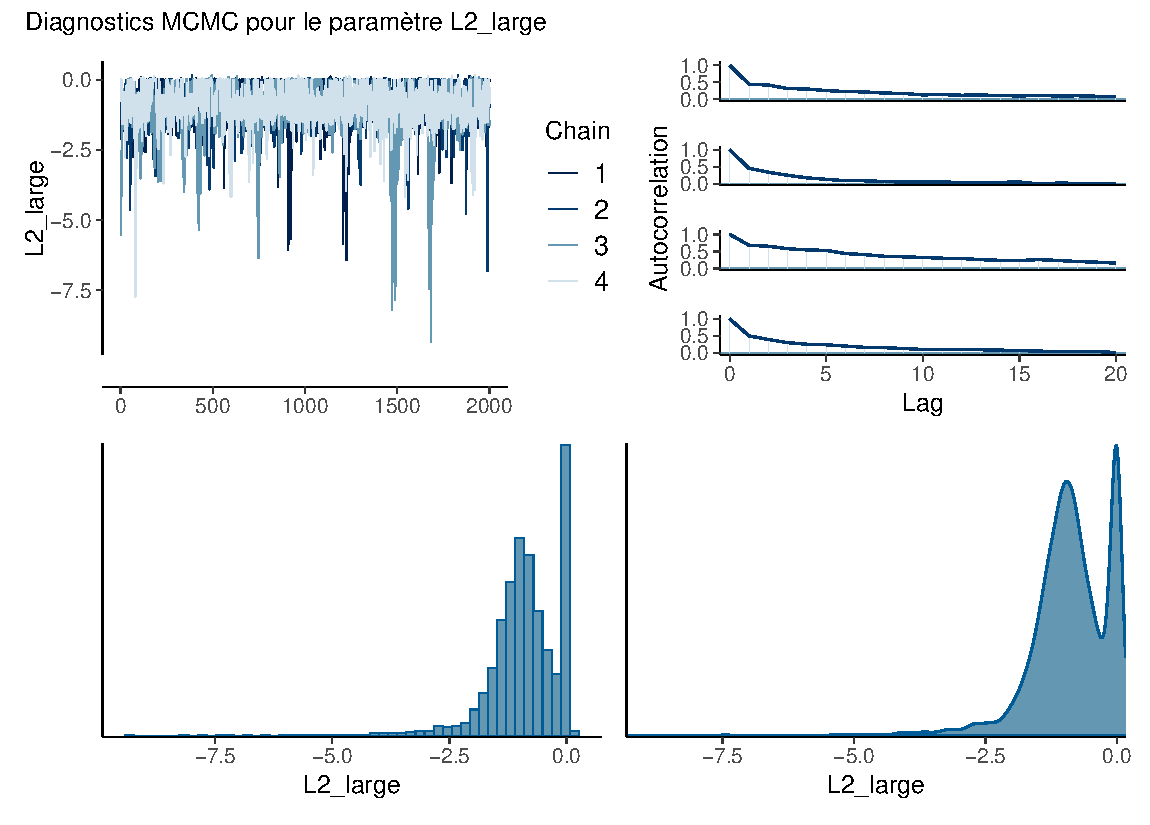
\includegraphics[scale=0.7]{diag_mcmc_ex.pdf}
	\caption[Diagnostics MCMC pour le paramètre \texttt{L2\_large}, modèle global]{%
	Exemple de diagnostics MCMC illustrés pour le paramètre \texttt{L2\_large}, sélectionné à partir du modèle global. De gauche à droite et de haut en bas~: (1) \textit{traceplot} des chaînes, un bon mélange est souhaité et se traduit par des chaînes entrelacées, similaires à un bruit blanc~; (2) fonction d'autocorrélation, une décroissance rapide vers zéro est souhaitée, ce qui indique une faible dépendance entre échantillons successifs~; (3) histogramme de la distribution \textit{a posteriori}, il doit contenir assez d'informations pour approximer la densité~; (4) courbe de densité estimée \textit{a posteriori}, l'axe \textit{x} de l'histogramme et de la courbe de densité est exprimé en taille d'effet standardisée. %Les pics ponctuels vers des valeurs extrêmes visibles sur le \textit{traceplot} reflètent les queues	lourdes du prior horseshoe et ne constituent pas un signe de non-convergence.
	}
	\label{fig:diag_mcmc_ex}
\end{figure}


Concernant l'approximation PSIS-LOO, 9 observations présentent un $\hat{k}$ de Pareto supérieur à $0.7$ (environ 10\,\% des observations), seuil au-delà duquel l'estimation PSIS est considérée peu fiable pour l'observation concernée \parencite{Vehtari2015Jul}. Ce résultat invite à interpréter les valeurs d'elpd avec prudence.


\subsection{Sensibilité au prior ($p_0$)}

Afin d'évaluer l'influence du prior sur les résultats, deux valeurs alternatives du paramètre $p_0$ ont été testées et comparées à la valeur de référence.

\medskip 

Les trois configurations conduisent à la sélection des mêmes quatre variables, dans le même ordre, avec des stabilités par \textit{fold} comparables. Les estimations \textit{a posteriori} des coefficients sont stables. Exprimés en fraction de la largeur de l'intervalle de crédibilité à 95\,\% du modèle de référence, les écarts normalisés $\delta_\text{norm}$ restent inférieurs à 10\% pour l'ensemble des paramètres et des deux valeurs alternatives testées (tableau~\ref{table:sensi_full}). %Le déplacement le plus important concerne \texttt{pT2Pv6} avec $p_0 = 20$ ($\delta_\text{norm} = 10.9\,\%$), ce qui demeure négligeable au regard de l'incertitude déjà présente sur ce coefficient.
Les signes et ordres de grandeur des effets sont identiques dans toutes les configurations.


\begin{table}[ht]
	\centering
	\begin{tabular}{lccccc}
		\hline
		& $\hat\beta_{\text{ref}}$ & $\hat\beta_{p_0=5}$ & $\delta_{\text{norm}} (\%)$ & $\hat\beta_{p_0=20}$ & $\delta_{\text{norm}} (\%)$ \\
		\hline
		Intercept     &  0.035 & 0.016  & 1.9 & 0.041  & 0.6 \\
		L2\_large     & -0.738 & -0.732 & 0.4 & -0.754 & 1.1 \\
		Sparc\_small  & -0.400 & -0.343 & 4.9 & -0.493 & 8.0 \\
		Sparc2        & -0.392 & -0.272 & 9.5 & -0.469 & 6.1 \\
		pT2Pv6        &  0.216 & 0.143  & 7.3 & 0.325  & 10.9 \\
		\hline
	\end{tabular}
	\caption[Analyse de sensibilité au prior $p_0$ pour le modèle complet]{Analyse de sensibilité des estimations \textit{a posteriori} au choix du paramètre $p_0$ du prior RHS. $\hat\beta_{\text{ref}}$ désigne la médiane \textit{a posteriori} du modèle de référence ($p_0 = 10$)~; $\delta_{\text{norm}}$ est l'écart normalisé en fonction de l'intervalle de crédibilité, tel que $\delta_{\text{norm}} = |\hat\beta_{p_0} - \hat\beta_{\text{ref}}|\,/\,(\text{largeur IC}_{95\%}^{\text{ref}}) \times 100$}
	\label{table:sensi_full}
\end{table} 

Sur le plan prédictif, les performances sont stables. Les valeurs d'elpd et d'\textit{accuracy} du modèle de référence et du sous-modèle restent du même ordre quelle que soit la valeur de $p_0$. On note toutefois qu'avec $p_0 = 20$, l'\textit{accuracy} du sous-modèle (0.689) est supérieure à celle du modèle de référence (0.667), tandis que les valeurs d'elpd demeurent proches. À l'inverse, avec $p_0 = 5$, les deux métriques convergent et les estimations des coefficients sont légèrement plus faibles. Cela indique une régularisation plus forte. La configuration $p_0 = 10$ semble donc être un compromis satisfaisant.

%
%
%avec p0 = 5
%stabilité 0.99,0.90,0.96,0.94 idem variables
%ELPD  — réf : -58.63  | sous-modèle : -55.67
%Accuracy — réf : 0.667 | sous-modèle : 0.656
%
%avec p0 = 20 
%stabilité 0.99, 0.94, 0.96, 0.93 idem variables
%
%ELPD  — réf : -57.72  | sous-modèle : -54.43
%Accuracy — réf : 0.667 | sous-modèle : 0.689
%
%L'analyse de sensibilité montre que le choix du prior p0 n'affecte ni l'ordre de sélection des variables, ni la stabilité du modèle, ni l'estimation des tailles d'effet (très très peu) ni ELPD/accuracy -> rédiger bien.
%
%Néamoins avec p0 = 20 : coeff plus grand et plus petit avec p0 = 5. Et avec p0=20 \textit{accuracy} du sous modèle plus grande mais elpd idem -> léger surapprentissage. Entre autre avec p0 = 10 hs prior fait son travail comme il faut pour éviter le surapprentissage et laisser exprimer le sgrands effets.
\section{Screening par tâche motrice}

La comparaison des modèles par tâche motrice via LOO-CV (%tableau~\ref{table:loo_compare}, 
voir figure~\ref{fig:loo_compare}) indique que le modèle restreint à la tâche PA est statistiquement équivalent au modèle complet ($\Delta$elpd $= -2.21$, $\widehat{SE} = 3.21$) selon le critère de l'erreur standard sur la différence d'elpd, tout en reposant sur un espace de variables nettement plus faible. En effet, le modèle PA présente un $p_\text{loo}$ (nombre de paramètres effectifs) plus faible que le modèle complet (8.08 vs 23.84), ce qui indique un modèle plus parcimonieux.

\medskip

Les modèles fondés sur les tâches Epow, ll\_ln et PS affichent des performances inférieures, avec des différences d'elpd qui excèdent leur erreur standard respective (voir figure~\ref{fig:loo_compare}). % mettre graph OU tableau
Ces résultats sont cohérents avec ceux de la section précédente, où les deux premières variables sélectionnées (\texttt{L2\_large}, \texttt{Sparc\_small}) sur le modèle complet appartenaient déjà à la tâche PA. La projection prédictive est donc conduite dans un second temps en restreignant l'espace des variables à cette seule tâche.


%\begin{tabular}{lrrrrrrrr} % garder éventuellement que jusqu'à se elpd loo
%	\hline
%	& elpd\_diff & se\_diff & elpd\_loo & se\_elpd\_loo & p\_loo & se\_p\_loo & looic & se\_looic\\
%	\hline
%	PA & 0.00 & 0.00 & -55.27 & 4.31 & 8.08 & 1.41 & 110.54 & 8.62\\
%	Full & -2.21 & 3.21 & -57.49 & 5.32 & 23.84 & 3.63 & 114.97 & 10.65\\
%	Epow & -5.57 & 4.63 & -60.84 & 2.79 & 5.94 & 0.61 & 121.68 & 5.57\\
%	ll\_ln & -6.87 & 4.02 & -62.14 & 2.14 & 5.33 & 0.53 & 124.28 & 4.28\\
%	PS & -7.54 & 4.39 & -62.81 & 4.53 & 12.92 & 2.78 & 125.62 & 9.06\\
%	\hline
%\caption[Statistiques LOO-CV par tâche motrice]{%
%	Statistiques LOO-CV pour chaque modèle par tâche motrice, classés par ordre 
%	décroissant de performance prédictive. $\Delta$elpd~: différence d'ELPD par 
%	rapport au meilleur modèle (PA)~; $\widehat{SE}$~: erreur standard associée~; 
%	elpd\_loo~: ELPD estimé par LOO-CV~; $p_\text{loo}$~: nombre effectif de 
%	paramètres, indicateur de complexité du modèle~; looic~: critère d'information 
%	LOO ($= -2 \times \text{elpd\_loo}$).}
%\label{table:loo_compare}
%\end{tabular}

\begin{figure}[ht]
	\centering
	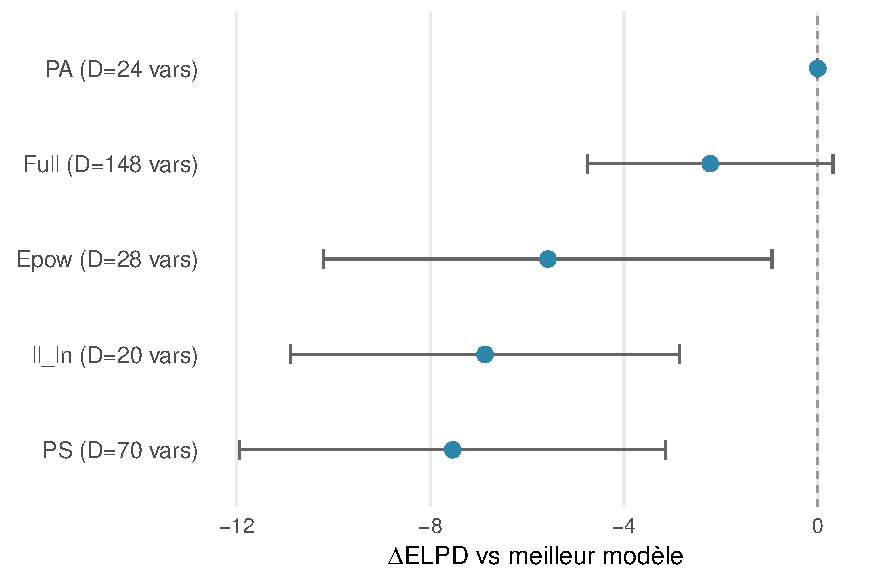
\includegraphics[scale=1]{loo_compare.pdf}
	\caption[Comparaison des modèles par tâche]{Comparaison des modèles par tâche selon l'elpd estimé par LOO-CV. Chaque point représente la différence d'elpd entre le modèle considéré et le meilleur modèle (PA, fixé à 0)~; les barres d'erreur indiquent	$\pm 1$ erreur standard sur cette différence. Une différence dont l'intervalle d'erreur standard chevauche zéro indique des performances prédictives statistiquement équivalentes au modèle issu de la tâche PA. Le modèle global (Full) est donc statistiquement équivalent à celui de la tâche PA.}
	\label{fig:loo_compare}
\end{figure}


\section{Sélection sur la tâche PA}

\subsection{Courbe elpd et sélection des variables} \label{sec:sel_PA}
La projection prédictive appliquée aux variables de la tâche PA conduit à la sélection de deux variables, \texttt{L2\_large} et \texttt{Sparc\_small}, retenues avec une stabilité de 0.99 chacune sur l'ensemble des \textit{folds} (voir \hyperref[fig:stab_PA]{Annexe D} pour le détail par variable). Le critère de l'erreur standard, la stabilité de sélection et le coude de la courbe elpd (figure~\ref{fig:elpd_PA}) convergent vers $k_\text{opt} = 2$. Il est important de noter que ces deux variables correspondent aux deux premières retenues lors de la sélection sur le modèle global (section~\ref{sec:sel_global}).




Les performances prédictives du sous-modèle sont comparables à celles du modèle de référence PA (sous-modèle vs référence~; elpd : $-52.82$ vs $-55.28$, \textit{accuracy} : 0.700 vs 0.700). La matrice de confusion indique 15 faux négatifs (classifié TD au lieu de TSA) et 11 faux positifs (classifié TSA au lieu de TD) sur 90 observations. Ces performances sont légèrement supérieures à celles obtenues sur le modèle global (section~\ref{sec:sel_global}), ce qui suggère que la restriction de l'espace des variables à la tâche PA réduit le bruit introduit par des variables peu informatives. On notera que l'elpd du sous-modèle est légèrement supérieur à celui du modèle de référence (figure~\ref{fig:elpd_PA}), ce qui peut refléter la régularisation induite par la réduction du modèle.

\medskip

%
%\begin{tabular}{lrr}
%	\hline
%	& 0 & 1\\
%	\hline
%	0 & 35 & 15\\
%	1 & 11 & 29\\
%	\hline
%\end{tabular}

Les estimations des coefficients \textit{a posteriori}, conditionnellement au modèle et aux données, sont présentées dans le tableau~\ref{table:inf_PA} et la figure~\ref{fig:mcmc_areas_cvvs_PA}. Les deux coefficients sont négatifs, avec des médianes respectivement de $-0.883$ et $-0.502$, et une incertitude réduite sur le signe des effets malgré une incertitude importante sur leur taille. Ces estimations sont proches de celles obtenues lors de la sélection sur le modèle complet, avec des écarts relatifs sur les médianes de 16\,\% pour \texttt{L2\_large} et 20\,\% pour \texttt{Sparc\_small}.

\begin{figure}[h!]
	\centering
	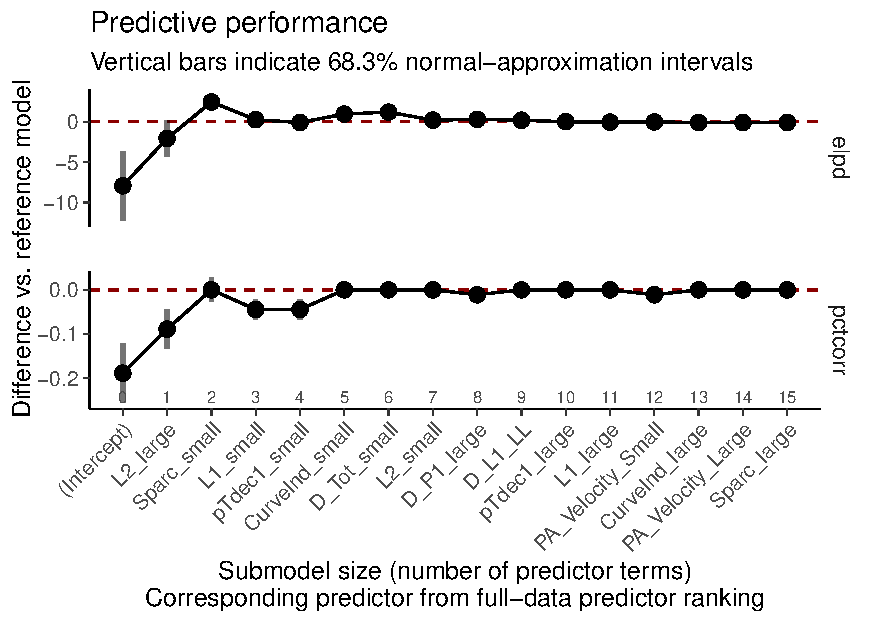
\includegraphics[scale=1]{elpd_PA.pdf}
	\caption[Courbes elpd et d'\textit{accuracy} issues du modèle de référence PA]{Courbes de l'elpd et de l'\textit{accuracy} issues du modèle de référence PA, en fonction du nombre de variables incluses dans le sous-modèle, obtenues par projection prédictive avec validation croisée. Chaque point représente la différence d'elpd/d'\textit{accuracy} entre le sous-modèle et le modèle de référence. Les barres d'erreur indiquent l'incertitude à $\pm 1$ erreur standard. Une différence proche de zéro indique des performances prédictives équivalentes au modèle de référence.}
	\label{fig:elpd_PA}
\end{figure}

\begin{figure}[h!]
	\centering
	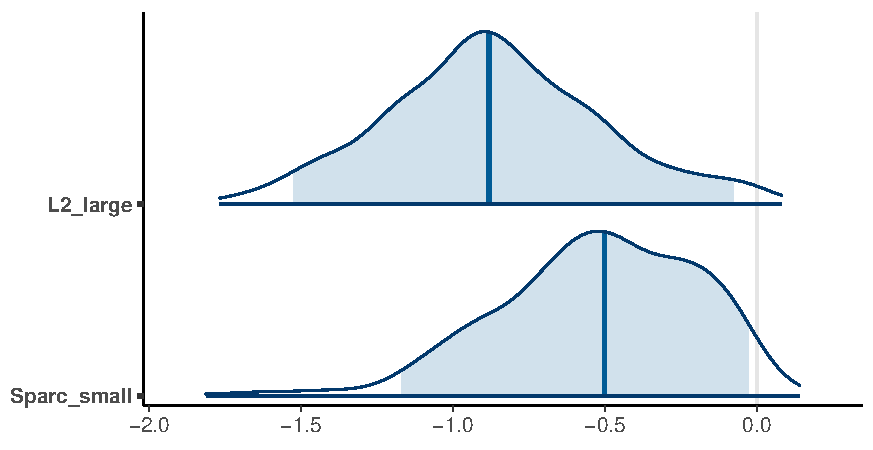
\includegraphics[scale=0.9]{mcmc_areas_cvvs_PA.pdf}
	\caption[Distributions \textit{a posteriori} du sous-modèle réduit à partir du modèle de référence PA]{Distributions \textit{a posteriori} des coefficients de régression du sous-modèle à deux variables à partir du modèle de référence PA. Pour chaque paramètre, la barre verticale bleue indique la médiane \textit{a posteriori} et la zone bleue représente l'intervalle de crédibilité à 95\,\% (IC$_{95\%}$). Conditionnellement au modèle et aux données, la valeur du paramètre a 95\,\% de chance de se situer dans cet intervalle.}
	\label{fig:mcmc_areas_cvvs_PA}
\end{figure}


\begin{table}[ht]
	\centering
	\begin{tabular}{lcccc}
		\hline
		& Médiane & $\text{IC}_{95\%}$ & $\text{P}(\beta_j < 0)$ & $\text{P}(\beta_j > 0)$ \\
		\hline
		Intercept      &  -0.011 & $[-0.463 \,;\, 0.463]$ & 0.52 & 0.48 \\
		L2\_large      & -0.883 & $[-1.524 \,;\, -0.076]$ & 0.99 & 0.01 \\
		Sparc\_small   & -0.502 & $[-1.169 \,;\, -0.028]$ & 0.97 & 0.03 \\
		\hline
	\end{tabular}
	\caption[Estimations \textit{a posteriori} du sous-modèle réduit à partir du modèle de référence PA]{Estimations \textit{a posteriori} des coefficients du sous-modèle à deux variables à partir du modèle de référence PA. La médiane et l'intervalle de crédibilité à 95\,\% (IC$_{95\%}$) résument la distribution \textit{a posteriori} de chaque coefficient~; $\text{P}(\beta_j < 0)$ et $\text{P}(\beta_j > 0)$ indiquent la probabilité \textit{a posteriori} que le coefficient soit négatif ou positif, respectivement (probabilité de direction).}
	\label{table:inf_PA}
\end{table}

\subsection{Diagnostics MCMC et approximation PSIS-LOO}

Les diagnostics MCMC (voir \hyperref[fig:diag_mcmc_ex_PA]{Annexe E}) ne révèlent pas de problème de convergence et l'ensemble des paramètres affiche un $\hat{R} < 1.01$ ainsi qu'une taille effective d'échantillon > 400. L'approximation PSIS-LOO est fiable pour l'ensemble des observations. Aucun $\hat{k}$ de Pareto ne dépasse le seuil de $0.7$, ce qui contraste avec les résultats obtenus sur le modèle global et renforce la confiance dans les estimations d'elpd utilisées pour la sélection avec le modèle de référence PA. 


\subsection{Sensibilité au prior ($p_0$)}
Deux valeurs alternatives du paramètre $p_0$ ont été testées et comparées à la valeur de référence ($p_0 = 5$). Les trois configurations conduisent à la sélection des mêmes deux variables, dans le même ordre, avec des stabilités par \textit{fold} identiques (0.99 et 0.99 dans toutes les configurations). Les estimations \textit{a posteriori} sont stables : les écarts normalisés $\delta_{\text{norm}}$ sont inférieurs à 4\,\% pour l'ensemble des paramètres (tableau~\ref{table:sensi_PA}).

\medskip 

Sur le plan prédictif, les performances restent globalement stables. Avec $p_0 = 10$, on observe néanmoins que l'\textit{accuracy} du modèle de référence augmente (0.711) alors que celle du sous-modèle ne suit pas (0.700), tandis que les valeurs d'elpd évoluent peu. Cela suggère un léger surapprentissage du modèle de référence. 

\begin{table}[ht]
	\centering
	\begin{tabular}{lccccc}
		\hline
		& $\hat\beta_{\text{ref}}$ & $\hat\beta_{p_0=3}$ & $\delta_{\text{norm}} (\%)$ & $\hat\beta_{p_0=10}$ & $\delta_{\text{norm}} (\%)$ \\
		\hline
		Intercept    & -0.011 & -0.033 & 2.4 & 0.008  & 2.0 \\ 
		L2\_large    & -0.883 & -0.898 & 1.0 & -0.939 & 3.9 \\
		Sparc\_small & -0.502 & -0.483 & 1.7 & -0.508 & 0.5 \\
		\hline
	\end{tabular}
	\caption[Analyse de sensibilité au prior $p_0$, modèle PA]{Analyse de sensibilité des estimations \textit{a posteriori} au choix du paramètre $p_0$ du prior RHS du modèle PA. $\hat\beta_{\text{ref}}$ désigne la médiane \textit{a posteriori} du modèle de référence ($p_0 = 5)$~; $\delta_{\text{norm}}$ est l'écart normalisé en fonction de l'intervalle de crédibilité, tel que $\delta_{\text{norm}} = |\hat\beta_{p_0} - \hat\beta_{\text{ref}}|\,/\,(\text{largeur IC}_{95\%}^{\text{ref}}) \times 100$}
	\label{table:sensi_PA}
\end{table}

%A p10 : stabilité idem (0.99, 0.99) 
%
%ELPD  — réf : -55.42  | sous-modèle : -52.47
%Accuracy — réf : 0.711 | sous-modèle : 0.700 -> léger signe d'overfitting, puisqu'avec prior plus souple \textit{accuracy} augmente mais pas elpd. De plus, l'accuracy du sous-modèle ne suit pas l'accuracy croissante de la référence, ce qui suggère que le gain en \textit{accuracy} à p10 est capté par la complexité du modèle de référence, pas par une meilleure généralisation du sous-modèle. Idem pour elpd : légère perte avec sous modèle. Sinon idem
%
%A p3 : stabilité idem (0.99, 0.99) 
%ELPD  — réf : -55.20  | sous-modèle : -53.04
%Accuracy — réf : 0.667 | sous-modèle : 0.689

%
%
%\begin{table}[ht]
%	\centering
%	\begin{tabular}{lccccc}
%		\hline
%		& Médiane ref p0 = 5 & Mediane p0 = 3 & Ecart relatif & Mediane p0 = 10 & Ecart relatif \\
%		\hline
%		Intercept      & -0.011 & -0.033 & 2 & 0.008 &\\
%		L2\_large      & -0.883 & -0.898 &  & -0.939 &\\
%		Sparc\_small   & -0.502 & -0.483 &  & -0.508 &\\
%		\hline
%	\end{tabular}
%	\caption[]{blabla ecart relatif def tel que |p0 diff - p0 ref|/p0 ref}
%	\label{table:sensi_PA}
%\end{table}

\subsection{Représentation dans l'espace des variables sélectionnées}

La figure~\ref{fig:espace_sel} représente les observations dans l'espace des deux variables sélectionnées, \texttt{L2\_large} et \texttt{Sparc\_small}. Les deux groupes forment des nuages distincts mais se chevauchent partiellement. Ce chevauchement est cohérent avec les performances prédictives observées (\textit{accuracy} de 0.700).


\begin{figure}[h!] % rajouter la droite de la regression ?
	\centering
	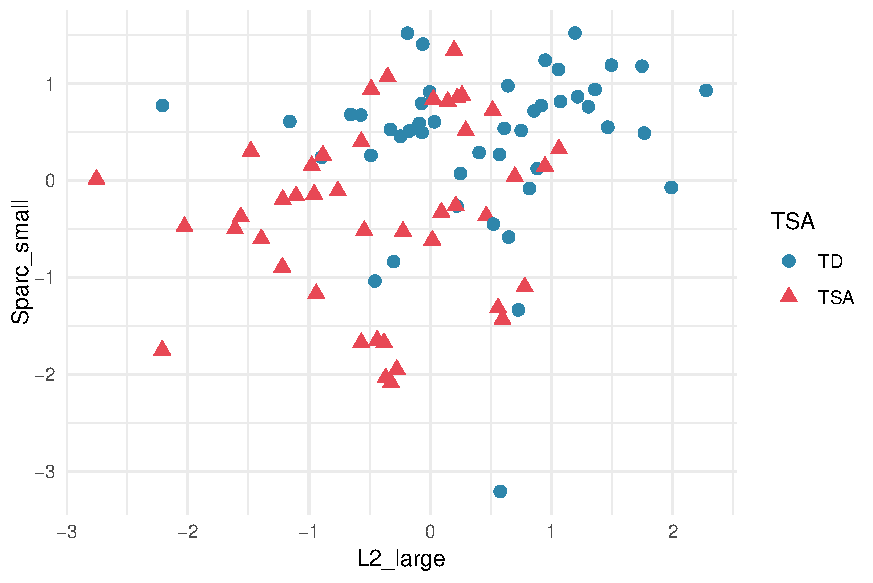
\includegraphics[scale=1.2]{espace_sel.pdf}
    \caption[Représentation des observations dans l'espace des variables 
	sélectionnées]{Représentation des observations dans l'espace des deux variables sélectionnées par projection prédictive sur la tâche PA (\texttt{L2\_large} et \texttt{Sparc\_small}). Les unités des axes sont en taille d'effet standardisée. }
	\label{fig:espace_sel}
\end{figure}

En conclusion, l'ensemble de ces analyses semble donc converger. Le modèle global produit une sélection stable malgré une incertitude élevée sur les différences d'elpd. Le screening par tâche motrice montre que le modèle restreint à la tâche PA est équivalent au modèle complet tout en reposant sur un espace de variables plus faible. La projection prédictive conduite sur ce sous-espace aboutit à un sous-modèle à deux variables, \texttt{L2\_large} et \texttt{Sparc\_small}, dont la sélection est très stable ($0.99$ sur l'ensemble des \textit{folds}) et cohérente avec les deux premières variables retenues sur le modèle global. Ces résultats sont peu sensibles au choix du prior $p_0$. De plus, les deux coefficients sont négatifs~: des valeurs plus élevées de \texttt{L2\_large} et de \texttt{Sparc\_small} sont associées à une probabilité réduite d'appartenir au groupe TSA, bien que l'incertitude sur la taille de ces effets demeure importante.

%
%\section{Performance prédictive}
%
%\subsection{Modèle global}
%
%\subsection{Modèle de référence PA}
%
%\subsection{Sous-modèle réduit}
%(+ tableau comparatif elpd / \textit{accuracy} LOO)
%(accuracy LOO, PPA, matrice de confusion...)


\chapter{Discussion}


la convergence des résultats entre le modèle PA et le modèle global malgré l'incertitude de ce dernier constitue un élément de validation indirecte de l'approche par décomposition


 Modèle complet (144 vars) → ELPD trop incertain pour conclure, mais tendance à 
 2-7 variables stable en sensibilité → justifie de décomposer par tâche → T1 domine
 les autres tâches au sens |elpd\_diff| > se\_diff → cv\_varsel sur T1 → 2 variables 
 (L2\_large, Sparc\_small) capturent l'essentiel avec elpd.diff = 2.45, se = 0.83 pour
 la taille 2 vs taille 3, ce qui est le seuil opti
 Dans cet échantillon, L2\_large et Sparc\_small constituent le sous-ensemble le plus 
 parcimonieux identifié par la sélection projective sur la tâche T1, avec une performance
 prédictive non distinguable du modèle de référence complet. La stabilité de leur sélection
 (cv\_proportions ~ 0.99) renforce leur statut de variables candidates pour des études 
 futures, sans pour autant permettre une inférence causale oun <- 94
 à la population TSA. + anticipation pointage
 Si Sparc\_small bien, Sparc\_large presque aussi bien, mais redondant donc non sélectionné
 Pour autant, L2\_large largement supérieur à L2\_small qui ne capture pas d'information



 intention au départ : visiblement on tend à dire que PA suffirait 
 + accent sur 2 variables, une liée à cible petite et une cible large
 spectre + tout les domaines enfants pas forcément différents
 enfants peut être en difficulté sur certaines tâches pour les uns, d'autres pour d'autres
 %kmeans ? -> si clusterisation similaire imposée PCA/kmeans ?



on a identifié des biomarqueurs moteurs de façon certaine, en éliminant bruit et redondance, mais modéré dans leur capacité à prédire quoi 
 
 
Age et sexe pas informatives : c'est normal !! puisque jeu de données équilibré, contrairement à la population général 

\section{Interprétation des variables sélectionnées}
Résultat principal 
L2 large + sparc small -> augmentation de la variable diminue proba de prédire TSA. Rapporter en odd ratio pour interprétation.
Sparc\_small/L2large : qu'est-ce qu'elles traduisent de différent
Fluidité : à quoi associé en terme de controles smoothness motor control...
Idem pour longueur de tâche
bioméca + intégrationsenso visuo/motrice

L2\_large distance plus courte, lien parkinson etc

Tâche PA  

Résultat secondaire
On peut regarde les variables sparc2 et pT2Pv6 du modèle réduit à partir du modèle de référence global, car stabilité ++ même si incertitude sur l'information que ça apporte. Rapporter en odd ratio pour interprétation.



Si accuracy modérée, c'est parce que bcp de sujet sont entre 2 -> correspond avec l'idée de spectre. Il y a des cas extrêmes qu'on classifie très bien, uniquement sur les marqueurs moteurs. 

Ce qui semble prédire : fluidité, donc plutôt sur des mouvement en feedforward et long (parce que peut être que quand TSA ils le font justement moins en feedforward). Et distance quand accuracy peu importante. Les composantes d'anticipation ne semble pas amener de l'information ?
(lien avec la littérature sur la motricité fine et le TSA)
\section{Apport de l'approche bayésienne}
(par rapport à une régression classique)
\section{Limites}
(taille d'échantillon, na.omit, généralisabilité, k pareto sur modèle réduit à partir ref globale, incertitude)




% Conclusion
\chapter{Conclusion}


\newpage
% Bibliographie
\pagestyle{empty}

\begingroup
\small % Ajuste la taille de la police
\setstretch{1.0} % Ajuste l'interligne
\printbibliography
%\bibliographystyle{apalike}
%\bibliography{biblio}
\endgroup


\newpage

\section*{Annexe A. Description de l'ensemble des variables}
\phantomsection \label{table:annexe_description_var}

\begin{table}[ht]
	\centering
	\begin{tabular}{lcccc}
	\end{tabular}
\end{table}

\newpage
\section*{Annexe B. \textit{Prior} et \textit{Posterior Predictive Checks}}\phantomsection \label{fig:ppc}

\begin{figure}[h!]
	\centering
	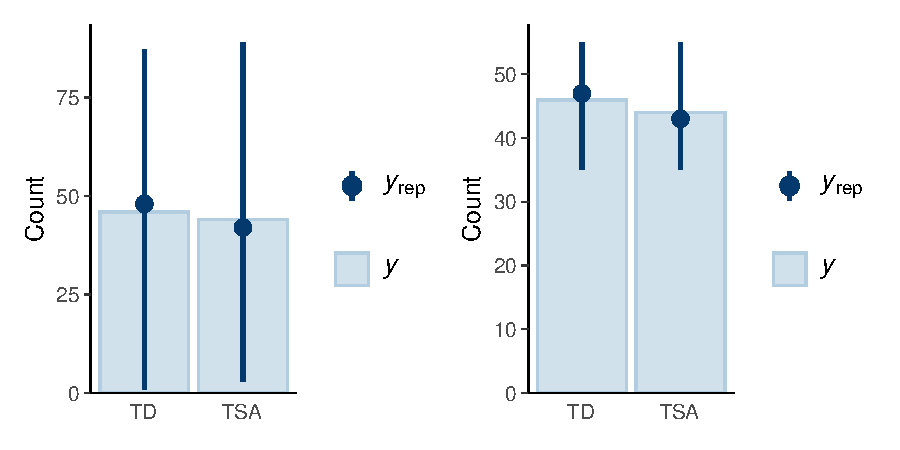
\includegraphics[scale=1]{ppc.pdf}
\end{figure}
\newpage
\section*{Annexe C. Stabilité de sélection des variables par \textit{fold} à partir du modèle de référence global}\phantomsection\label{fig:stab_ref}

\begin{figure}[h!]
	\centering
	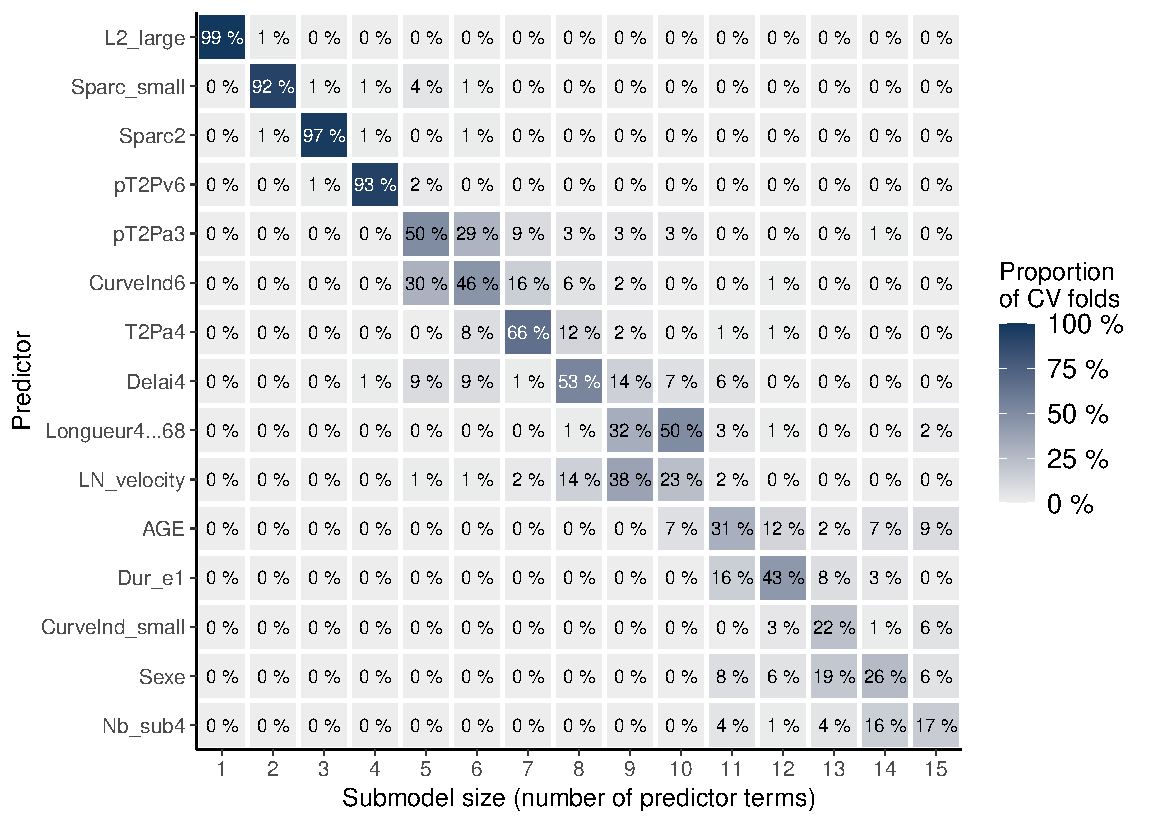
\includegraphics[scale=0.9]{stabilite_ref.pdf}ap
\end{figure}
\newpage
\section*{Annexe D. Stabilité de sélection des variables par \textit{fold} à partir du modèle de référence PA}\phantomsection\label{fig:stab_PA}

\begin{figure}[h!]
	\centering
	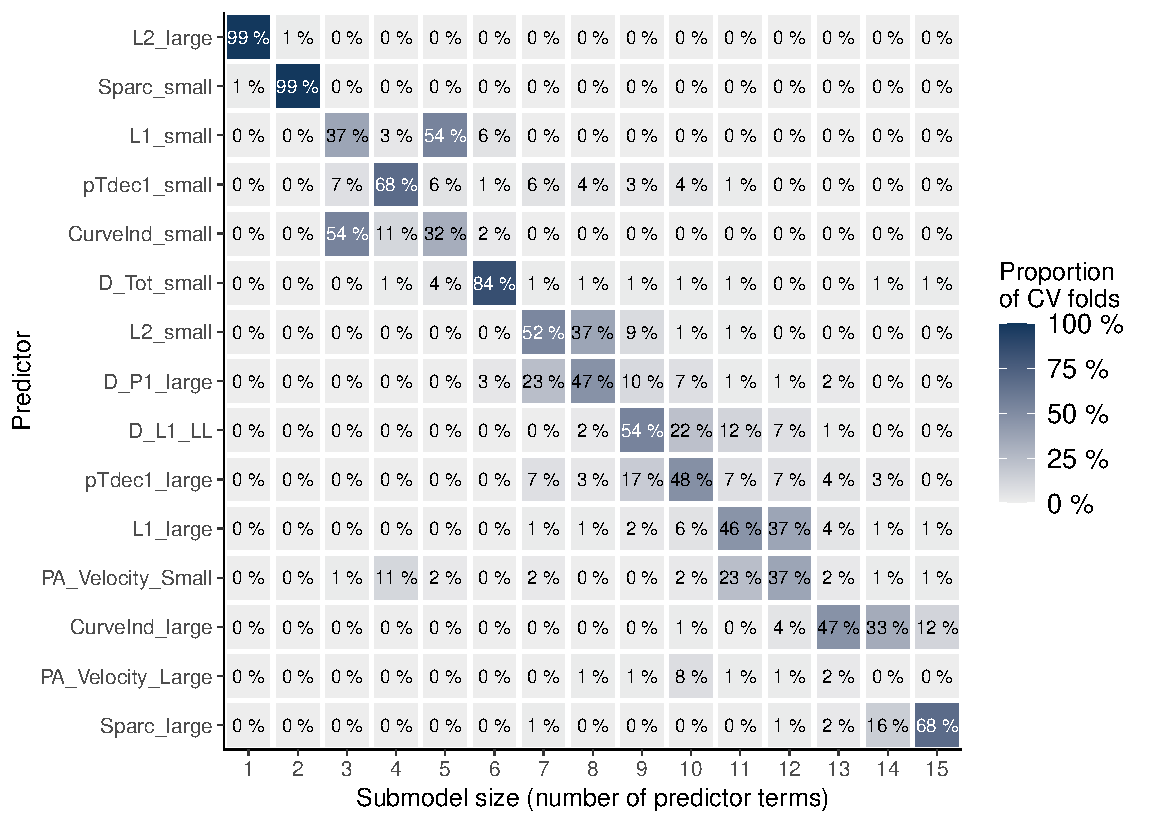
\includegraphics[scale=0.9]{stabilite_PA.pdf}
\end{figure}
\newpage
\section*{Annexe E. Représentation des deux composantes principales issues de l'ACP réalisée sur les 4 variables sélectionnées pour les sujet TSA }\phantomsection\label{fig:acp}

\begin{figure}[h!]
	\centering
	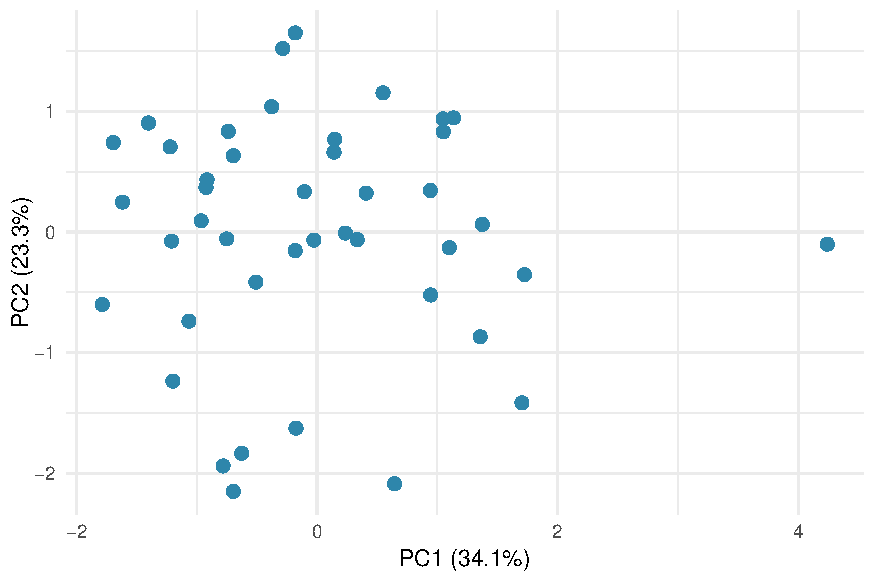
\includegraphics[scale=1]{acp.pdf}
\end{figure}




\newgeometry{hmargin=1.5cm, vmargin=1.5cm}
\begin{wrapfigure}[3]{r}{6cm}
	\vspace{-10pt}
	\centering
	\begin{tabular}{m{2.2cm} >{\centering\arraybackslash}m{0.4cm} m{2.0cm}} 
		
\includegraphics[height=2cm]{images/ens.pdf} 
		& 
		{\vrule height 0.6cm} 
		&  
		
\includegraphics[height=2cm]{images/R1.pdf}
	\end{tabular}
\end{wrapfigure}
\noindent\normalsize{Ecole normale supérieure de Rennes}
\vspace{0.01\baselineskip}

\noindent\normalsize{Département Sciences du sport et éducation physique}
\vspace{0.01\baselineskip}

\noindent\normalsize{Année 2025-2026 -- Diplôme de l'ENS -- 1A}

\hrulefill

\begin{center}
  {\bf{\Large{Identification des marqueurs de motricité fine les plus caractéristiques des TSA chez l'enfant : Approche bayésienne par projection prédictive }}}
\end{center}
\vspace{0.01\baselineskip}
{\bf{\textit{Présenté par : Romain MARTINIE}}}

\textit{Sous la direction de : Laetitia FRADET (Université de Bretagne-Sud) \& Germain FAITY (ENS 2SEP)}
\singlespacing
\small{{\bf{RÉSUMÉ}}}

\footnotesize{{\bf{Objectif}} : Identifier les marqueurs de motricité fine les plus caractéristiques des TSA chez l'enfant pour améliorer la compréhension du phénotype moteur et explorer des pistes diagnostiques complémentaires. 
	
{\bf{Méthode}} : Des marqueurs de motricité fine de 90 enfants (46 TD, 44 TSA) ont été analysés via une approche bayésienne par projection prédictive. Un modèle de référence intégrant 144 variables issues de quatre tâches motrices a été décomposé pour identifier la tâche la plus discriminante. Une sélection de variables a ensuite été opérée sur le sous-modèle retenu. 

{\bf{Résultats}} : La tâche de Pointage Anticipation (PA) a été sélectionnée comme la plus informative. Deux variables suffisantes pour reproduire la capacité prédictive du modèle ont été identifiées : une codant l'amplitude du mouvement et une la fluidité, avec une précision similaire à ce qui est rapporté dans la littérature (0.700).

{\bf{Discussion}} : Les coefficients négatifs associés aux variables sélectionnées traduisent une hypokinésie et un déficit de fluidité chez les enfants TSA, ce qui semble être causé par des altérations des mécanismes de planification en \textit{feedforward} potentiellement liés au cervelet et aux ganglions de la base. 

{\bf{Conclusion}} : Bien qu'exploratoires en raison du contexte de haute dimensionnalité, ces résultats pointent vers une réduction de l'amplitude du mouvement et de la fluidité lors de tâches de pointage comme les marqueurs de motricité fine les plus caractéristiques des TSA au sein de cet échantillon.

\medskip

{\bf{Mots-clefs : TSA, motricité fine, inférence bayésienne, projection prédictive, contrôle proactif. }}

\vspace{1.5\baselineskip}


\small{{\bf{ABSTRACT}}}

\footnotesize{{\bf{Objectives}}: To identify the most characteristic fine motor markers of ASD in children to improve the understanding of the motor phenotype and explore complementary ways of diagnostic.

{\bf{Method}}: Fine motor markers from 90 children (46 TD, 44 ASD) were analyzed using a Bayesian projective prediction approach. A reference model incorporating 144 variables from four motor tasks was decomposed to identify the most discriminant task. Variable selection was then performed on the selected sub-model. 
	
{\bf{Results}}: The Pointing task with Anticipation (PA) was selected as the most informative. Two variables sufficient to replicate the model's predictive power were identified: one encoding movement amplitude and one encoding smoothness, achieving an accuracy similar to that reported in the literature (0.700).

{\bf{Discussion}}: The negative coefficients associated with the selected variables reflect hypokinesia and a lack of smoothness in children with ASD, potentially caused by alterations in feedforward planning mechanisms linked to the cerebellum and basal ganglia.

{\bf{Conclusion}}: Although exploratory due to the high-dimensional context, these results point to reduced movement amplitude and smoothness during pointing tasks as the most characteristic fine motor markers of ASD within this sample.}

\medskip

{\bf{Keywords: ASD, fine motor skills, Bayesian inference, projective prediction, feedforward control.}}

\vspace{1\baselineskip}

{romain.martinie@ens-rennes.fr}

\end{document}
